\documentclass[9pt,pdftex]{beamer}
\setbeamertemplate{section in toc}[sections numbered]
\setbeamertemplate{subsection in toc}%
{\leavevmode\leftskip=3em\rlap{\hskip-2em\inserttocsectionnumber.\inserttocsubsectionnumber}\inserttocsubsection\par}
% use git: import repository as new project in eclipse: http://www.eclipse.org/forums/index.php/t/226301/
\usepackage[utf8]{inputenc}
\usepackage[english]{babel}
\usepackage{amsfonts, amsmath, amssymb}
\usepackage[bf,small, format=plain]{caption}
\usepackage{color}
\usepackage{graphicx}
\usepackage{tikz,tikzscale,pgfplots,grffile}
\usepgflibrary{arrows}
\usetikzlibrary{plotmarks}
%\usepackage{multirow}
% \usepackage{paralist}
%\usepackage[colorinlistoftodos]{todonotes}
%\usepackage{biblatex}
%usepackage[nolist,nohyperlinks]{acronym}
%\usepackage{amstext}
%\usepackage{hyperref} 
%\usepackage{comment}
%\usepackage{subcaption}
%\renewcommand*{\figureautorefname}{fig.}
%\renewcommand*{\equationautorefname}{eq.}
\usepackage{bm}
\usepackage{comment}
%\usepackage{beamerthemeshadow}
%\usepackage{tikz}
%\usepackage{pgfplots}
%\usepackage{ulem}
%\usepackage[lofdepth,lotdepth]{subfig}
%\newenvironment{figure*}%
%{\begin{figure}}
%{\end{figure}}
%\usepackage[style=mla,babel=hyphen,backend=biber]{biblatex}
% CSE-Beamer-Styles:
%\usepackage[conference]{beamertheme_sccstalk}
\usepackage[lecture]{beamertheme_sccstalk}
\usepackage{beamercolorscheme_sccs}
\usepackage{beamerfontthemestructurebold}
\setcounter{tocdepth}{3} 
%some useful commands
%\newcommand{\der}[2]{\frac{\text{d}#1}{\text{d}#2}}
\title{BGCE Project: CAD -- Integrated Topology Optimization}
\subtitle{BGCE First Milestone Meeting}
\author[E. Wannerberg, B. Rüth] {S. Joshi, J.C. Medina, F. Menhorn, S. Reiz, \textit{B. Rüth}, \textit{E. Wannerberg}, A. Yurova} %[displayed in footer]{displayed on title page}
\date{\today}
\institute{Technische Universität München}
\newtheorem*{rem}{Remark}

\begin{document}
\titlepage
\begin{frame}{Contents}
\tableofcontents
\end{frame}

\begin{frame}{Overview: Workflow}
	\begin{overlayarea}{\textwidth}{.1\textheight}
	\only<1>{What the user sees}
    \only<2>{CAD design including specification of loads and fixtures}
	\only<3>{Voxelized topology}
	\only<4>{Optimized topology}
	\only<5>{Surface extraction}
	\only<6>{Fit B-Spline surface}
	\end{overlayarea}
	\begin{overlayarea}{\textwidth}{.9\textheight}
    \begin{center}
		\begin{tikzpicture} 
        \uncover<1->{
        \node at (0,3)[inner sep=0pt](N1)
                {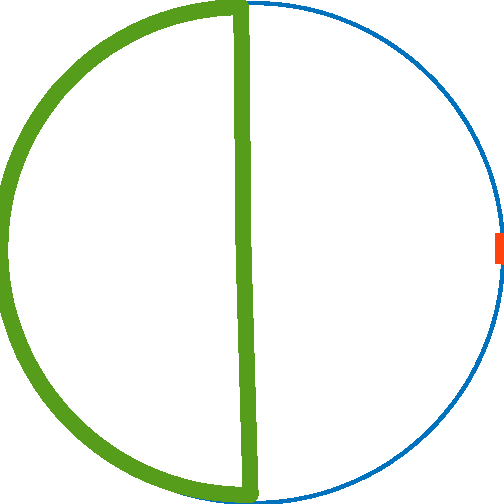
\includegraphics[width=2cm]{Pictures/1CAD_colored.pdf}};
		}
        \uncover<1->{
        \node at (0,0)[inner sep=0pt](N5)
		{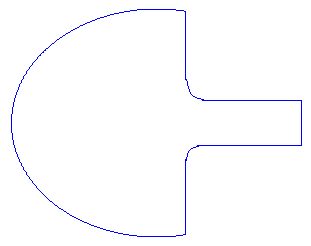
\includegraphics[width=2.2cm,height=2.2cm]{Pictures/End.png}};                        
		}        
        \uncover<1-1>{
       \draw[thick,->] (N1) -- (N5); 
		 }     
        \uncover<3->{
        \node at (4.5,3)[inner sep=0pt](N2)             
                {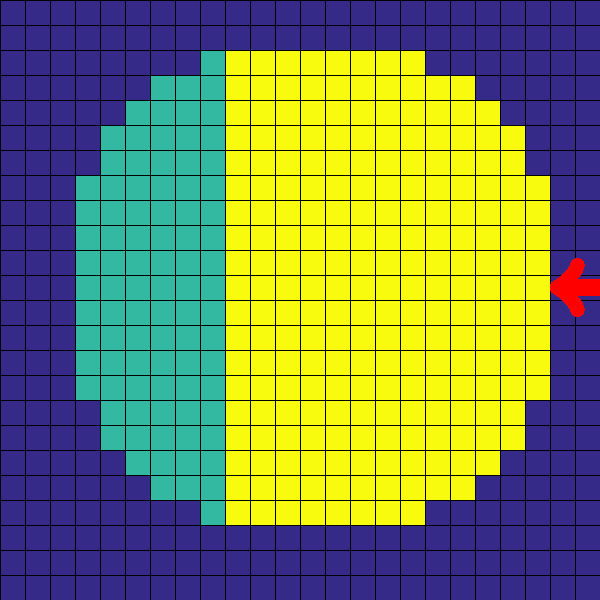
\includegraphics[width=2cm]{Pictures/4TPD.pdf}};
        \draw[thick,->] (N1) -- (N2);
        }
        \uncover<4->{
        \node at (9,1.5)[inner sep=0pt](N3) 
                {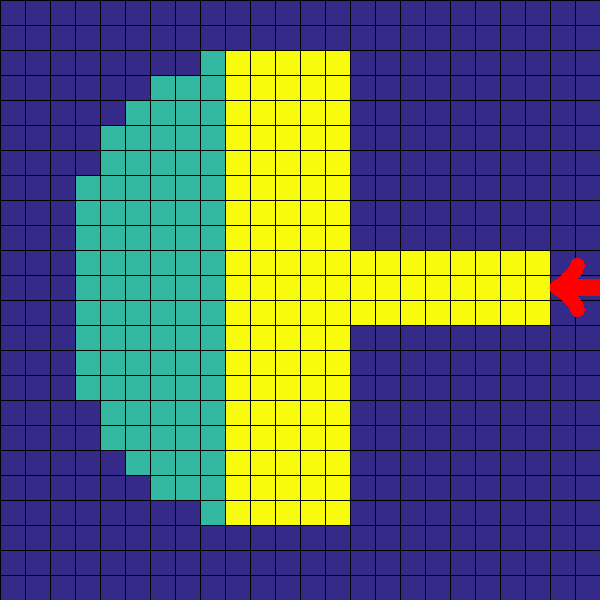
\includegraphics[width=2cm]{Pictures/5TOPOPT.pdf}};
        \draw[thick,->] (N2) -- (N3); 
        }
        \uncover<5->{
        \node at (4.5,0)[inner sep=0pt](N4)
                {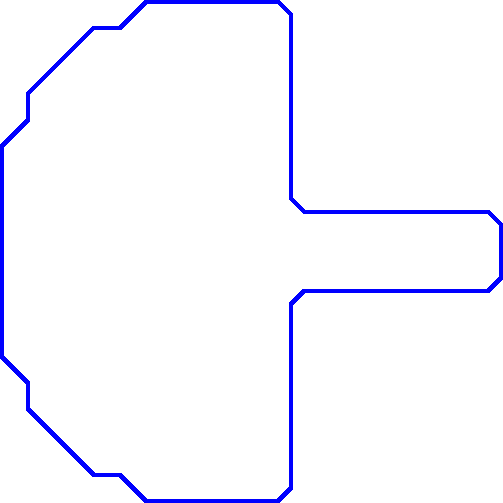
\includegraphics[width=2cm]{Pictures/7MC.pdf}};
        \draw[thick,->] (N3) -- (N4);
        }
        \uncover<6->{\draw[thick,->] (N4) -- (N5); 
        }

        \end{tikzpicture}
	\end{center}
	\end{overlayarea}

\end{frame}


\section{CAD overview}
\label{sec:CADbackg}
%interaction with it, programs, geometry represenations, datastructures, formats etc., maybe even history if we're overkill
\Acf{CAD} refers to the process of designing a product using a computer system. Before \ac{CAD} applications were used, products were designed using a sketch board. It was a challenge to incorporate changes in the construction drafts as well as to keep documentations up to date; hence, it was no surprise that \ac{CAD} systems spread rapidly across all design development branches. \Ac{CAD} is now of irreplaceable use in architecture, mechanical, electrical and civil engineering.

Depending on the discipline, different requirements are set on the virtual model. One may imagine that in a civil engineering model of a building a 2D floor plan is often sufficient; however, in the design of a mechanical motor a 3D model is always necessary. Given these circumstances, various \ac{CAD} software bundles evolved in the different disciplines with completely different modelling approaches. Besides the geometry representation additional parameters, such as material properties or manufacturing information, are stored. In order to move between different data structures standardized exchange interfaces are commonly used. 

This section presents the relevant geometrical and computational aspects of \ac{CAD} for the project; for a more thorough introduction we refer to \cite{sarcarCAD}.

\subsection{Geometry representations}
In general, two different ways of describing a geometry are used in \ac{CAD} systems: a \acf{CSG} or a \acf{BREP}. Other approaches, such as a complete voxelised geometry are not common due to extensive memory consumption.
\subsubsection{\Acl{CSG}}
\begin{figure}
\centering
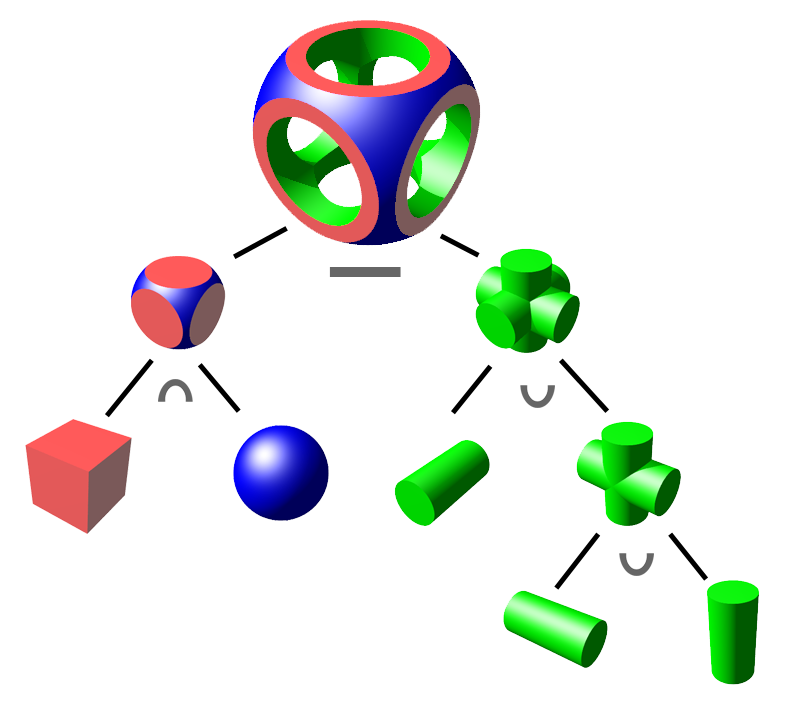
\includegraphics[width=0.5\textwidth]{Pictures/Csg_tree.png}
\caption{\ac{CSG} object tree. The picture shows the construction of a complex object from a cube, a sphere, and a set of cylinders. Figure taken from \cite{WikipediaCSG}.}
\label{fig:csg_tree}
\end{figure}
One way of representing a geometry in \ac{CAD} is the approach of \ac{CSG}\todo{long form at the beginning of the subsubsection?}. The basic idea is to start from a set of primitives, e.g. spheres, cylinders and/or cubes. Basic Boolean operations link these primitives towards a complex geometry, as illustrated in \autoref{fig:csg_tree}.

Key advantages of this format is the precise representation using very little storage memory. However, not all desired forms can be represented by \ac{CSG} and hence, a second type of geometry description is needed. 
\subsubsection{\Acl{BREP}}
A different kind of modelling approach is the \ac{BREP}\todo{long form at the beginning of the subsubsection?}. Instead of storing the geometry information as geometrical objects, \ac{BREP} formats only save the boundary surface of the body. The interior is assumed to be uniformly filled. Especially in complex geometries, this approach simplifies the model to such an extent, that the amount of data becomes much easier to handle. Surfaces can then be for example stored as a set of triangles (as in \ac{STL} files, see \autoref{subsub:STL} below) or in \ac{NURBS} \acsp{patch} (see \autoref{sec:NURBS}).
Furthermore, holes in the body are made possible by saving the surface normal of the respective boundary. 

By the boundary representation arbitrary geometries can be created. While the data sizes are commonly larger than in \ac{CSG} representation, \ac{BREP} files are usually easier to work with. One also has to keep in mind, that non-physical geometries can result from \ac{BREP} formats through a not closed surface.
\subsection{Data exchange interfaces}
\ac{CAD} software programs usually use their own data formats; in order to exchange models standardized interface formats have been developed. Geometric models are compressed to certain geometry descriptions; transferring additional information, such as material properties or manufacturing information, is in general a difficult task and in some exchange file formats even prohibited. A few common exchange file types are described below, as also compared in \cite{STL}.
\subsubsection{\acs{STL} file format} \label{subsub:STL}
The \acf{STL} file format describes the model only by its boundary and is thus a \ac{BREP} format. The idea behind its files is simple. The geometric model is discretized into a cloud of points, where sets of three vertices form a triangle; hence, a connected surface of triangles emerges which describes the geometry. The procedure is shown in \autoref{fig:STL} for a two dimensional circle.  
\begin{figure}
\centering
   \scalebox{0.4}{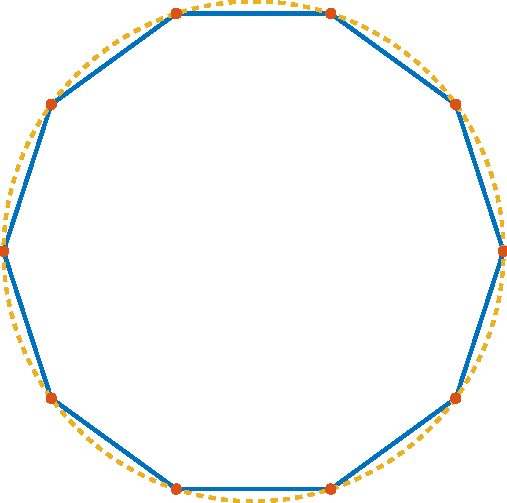
\includegraphics{Pictures/STL.pdf}}\\
   \caption{\ac{STL} discretization for a circle, self-made in MATLAB \cite{MATLAB}. Note that the circle cannot be exactly represented by the vertices and edges.}
   \label{fig:STL}
\end{figure}
The aforementioned triangles boil down to lines in two dimensions. The advantages and disadvantages of this approach become clear: It can be applied to an arbitrary geometry, but accuracy causes difficulties. In order to transfer high precision geometries many vertices are necessary, resulting in big files. Still, as is illustrated in the figure, a perfect circle can never be represented. 

ASCII \ac{STL} files begin with a name and the data on the triangles is constructed as follows: 
\begin{itemize}
\item a facet normal pointing outward
\item a sequence of vertex coordinates
\end{itemize}
As this is the only information provided, no additional data such as material properties are transferred through \ac{STL} files, reducing file size but also range of usage.
\subsubsection{\acs{STEP} and \acs{IGES} file formats}
To overcome issues of insufficient precision also more elaborate exchange formats exist; these save e.g. a circle as a parameter where no discretization step is involved. Also, the possibility of passing additional parameter information (e.g. density, manufacturing information) is required by certain users. Popular file types that offer these two functionalities are \acf{STEP} and \acf{IGES} files. 

The \ac{STEP} file format is a newly developed \ac{CAD} data exchange standard and documented in the ISO 10303 norm. On the contrary to \ac{STL} files it uses a combination of \ac{CSG} and \ac{BREP} to store the geometry. Additional information (e.g. density) are passed through attribute sets that are stored besides geometry instances (e.g. a circle). A key disadvantage, however, is that \ac{STEP} files carry much redundant information \cite{STL}.


The \acl{IGES} is an American National Standard since 1981 to exchange graphics information. Similar to the \ac{STEP} format it uses a combination of \ac{CSG} and \ac{BREP} for the geometry representation. Instead of storing a set of manufacturing information as done in the \ac{STEP} file, the \ac{IGES} is build only to exchange graphics information. For example, the step file transfers a physical density information; in the \ac{IGES} format the only additional parameter store node coloring information. Consequentially, \ac{IGES} file sizes are significantly smaller compared to the \ac{STEP} file format \cite{STL}.

The \ac{IGES} file format contains five different sections: a \emph{Start}, \emph{Global}, \emph{Directory Entry}, \emph{Parameter Data} and \emph{Terminate} section. The \emph{Start} and \emph{Global} section are used for naming and part information. In the \emph{Directory Entry} section additional information like the node color is saved. The \emph{Parameter Data} section is used for storing the coordinate points; the \emph{Terminate} section signals the end of the file \cite{sarcarCAD}.


\subsection{Voxelization}
\label{sec: Voxelization}

\tododone[inline]{Severin: Describe the voxelization process. Explain concept of refinement.}
%what is voxelisation
As pointed out in section \ref{sec:TopOpt} a very common formulation of topology optimization deals with regions that are specified as filled or empty. The minimum compliance problem is then solved on a discretized grid; the most common one is a volume raster in the form of cubes - so called voxels. Since ToPy requires a voxel grid in their input format, the next step is to render the geometry with a 3D raster of voxels.  

As described in the previous section, the geometry shape and faces for each boundary condition type, are stored in OpenCascade through the internal data type \lstinline|TopoDSShape|. As one can see in the UML Diagram \ref{fig: umlCADToVoxel} the \lstinline|voxelise| function is called internally by \lstinline|CADTOVoxel| -- for the shape and each faces separately. The voxelisation is then performed as follows: 
\begin{enumerate}
\item In order to combine the 3D voxel raster consistently, a bounding box is introduced. As a consequence the same coordinate system is used and voxel numbers are consistent between different voxelization types (faces and shapes). 
\item In each dimension $2^n*l_d$ voxels are created, where $n$ is the user specified refinement level and $l_d$ is the size of the bounding box in the respective dimension $d$
\item Voxelization is performed with the OpenCascade  \lstinline|Voxel_FastConverter.hxx| class creating a \lstinline|VoxelShape|
\end{enumerate}
\tododone[inline]{OpenCascade TopoBoolDS shape}

Consequentially, a 3D boolean voxel raster is created for each type -- since boundary conditions may consist of more than one face, they are voxelized separately and lists of \lstinline|VoxelShape| are created. 

\begin{frame}
	\frametitle{Load and fixture specification}
	\begin{minipage}{0.85\textwidth}
	Boundary conditions required - how to specify?
		\begin{itemize}
		\item Current state: Manual specification
		\item Idea 1: Metafile before Voxelization step
		\end{itemize}
		
	\end{minipage}
	\begin{minipage}{0.14\textwidth}
		\begin{figure}
			\scalebox{0.08}{
\includegraphics{Pictures/1CAD.pdf}}\\
			\scalebox{0.08}{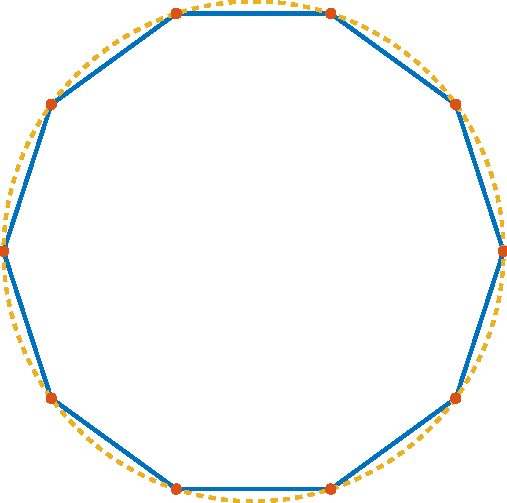
\includegraphics{Pictures/2STL.pdf}}\\
			\scalebox{0.08}{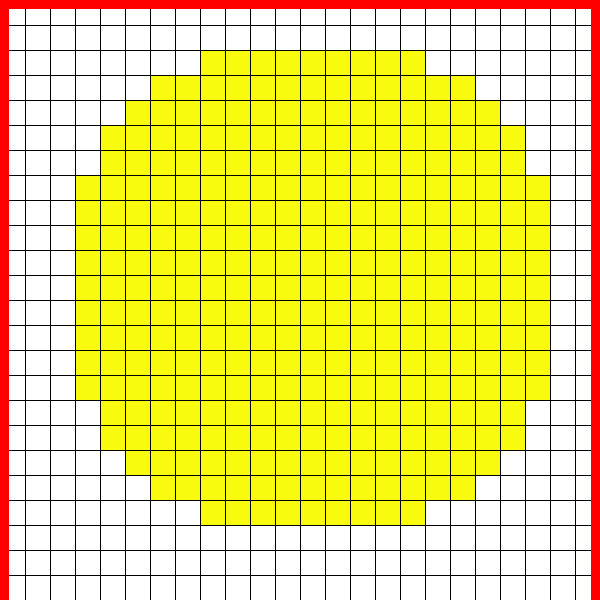
\includegraphics{Pictures/3VOXmark2.pdf}}\\
			\scalebox{0.08}{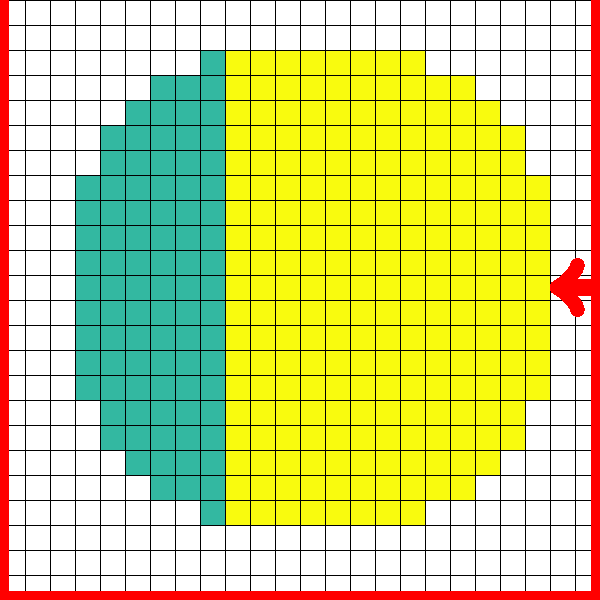
\includegraphics{Pictures/4TPDmark1.pdf}}\\
			\scalebox{0.08}{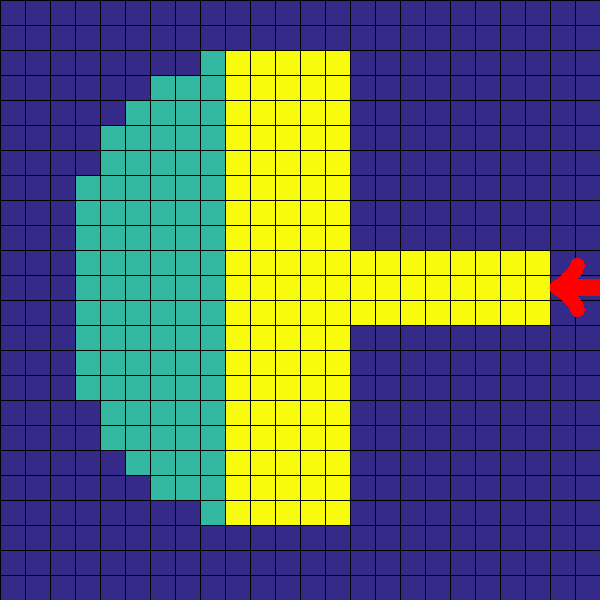
\includegraphics{Pictures/5TOPOPT.pdf}}\\
			\scalebox{0.08}{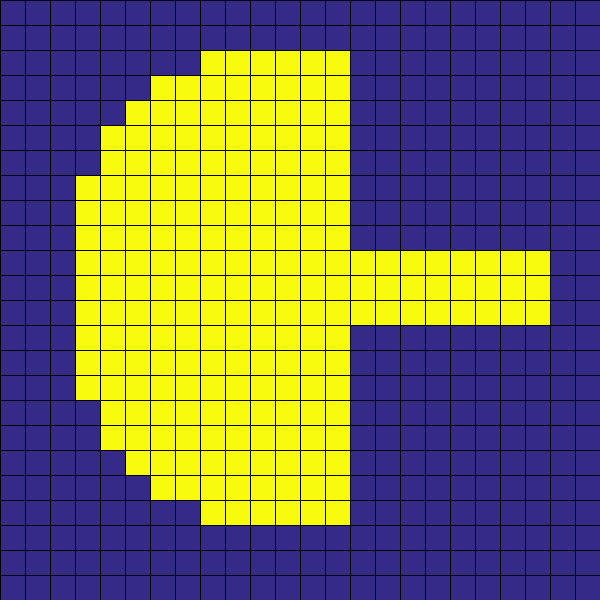
\includegraphics{Pictures/6TOPYOUT.pdf}}\\
			\scalebox{0.08}{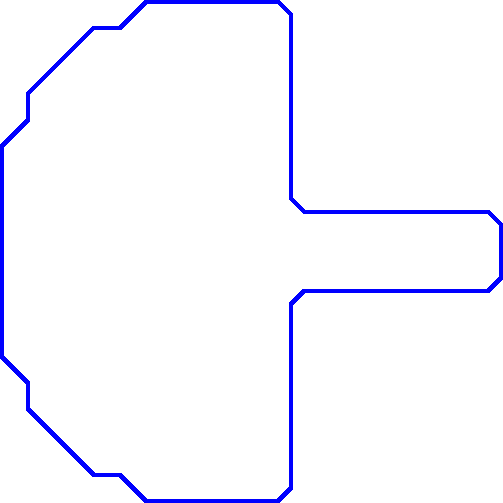
\includegraphics{Pictures/7MC.pdf}}
		\end{figure}
	\end{minipage}
\end{frame}


\setbeamertemplate{caption}{\raggedright\insertcaption\par}

\begin{frame}{Voxelized geometry}
\begin{itemize}
\item Done using OpenCascade  
\item Each region voxelized separately 
\end{itemize}
\vspace{0.4cm}
%\begin{enumerate}
%\item Active voxels (geometry)
%\item Fixture voxels
%\item Non-changing voxels
%\item Load voxels
%\end{enumerate}
\begin{minipage}{0.49\textwidth}
\begin{figure}
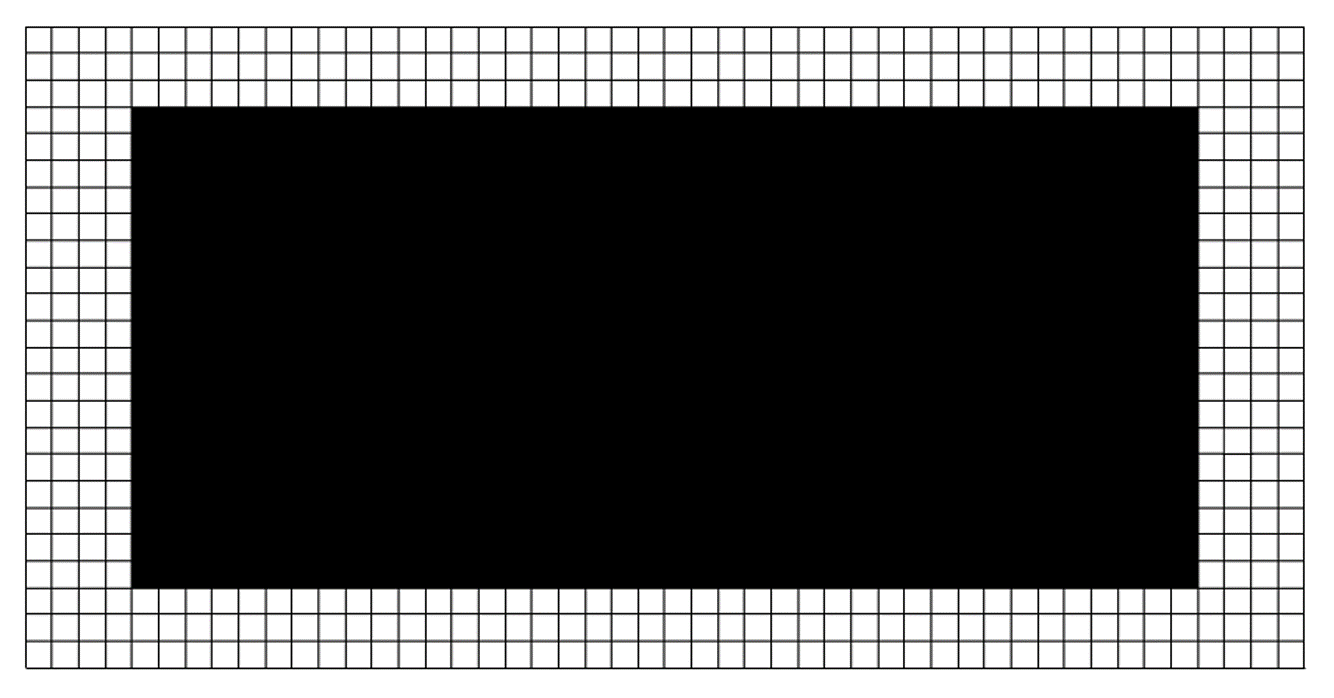
\includegraphics[width=.7\textwidth]{Pictures/Voxels/Active_2.png}
\vspace*{-2mm}
\caption{Participating voxels}
\end{figure}
\vspace{-0.6cm}
 \begin{figure}
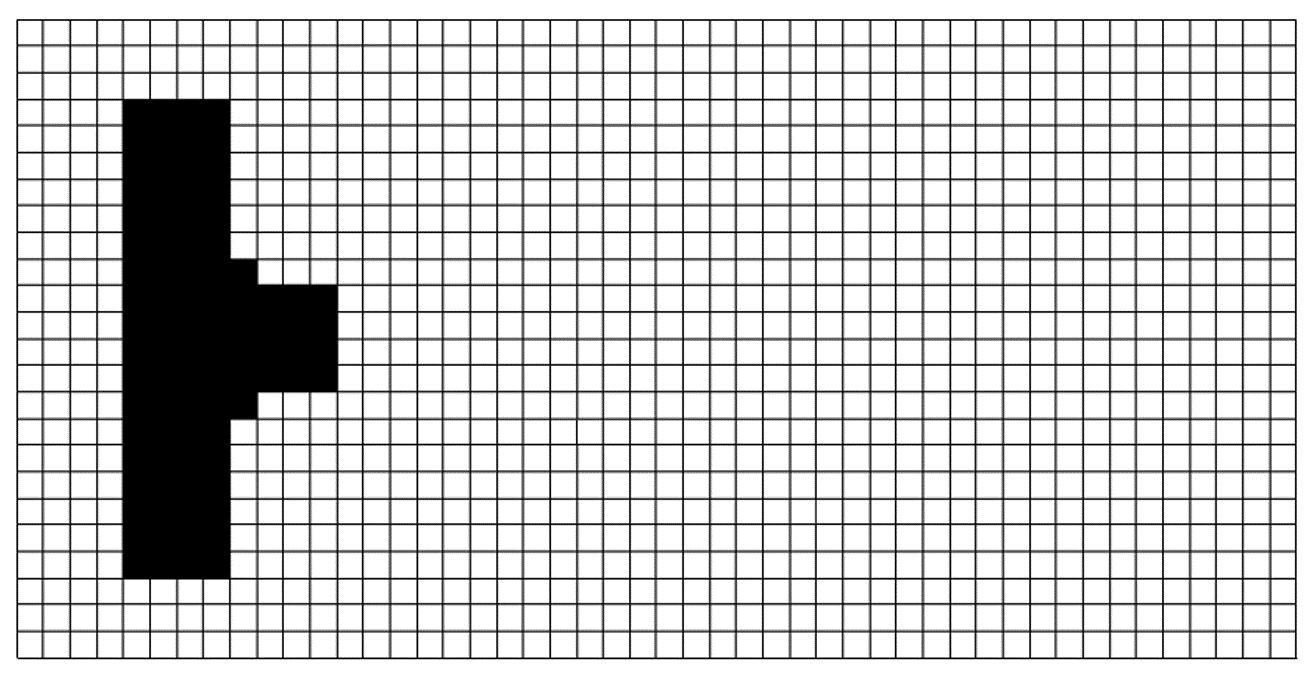
\includegraphics[width=.7\textwidth]{Pictures/Voxels/NonChanging.png}
\vspace*{-2mm}
\caption{Non-Changing Voxels}
\end{figure}
\end{minipage}
\hfill
\begin{minipage}{0.49\textwidth}
\begin{figure}

\includegraphics[width=.7\textwidth]{Pictures/Voxels/Fixture.png}
\vspace*{-2mm}
\caption{Fixture voxels}
\end{figure}
\vspace{-0.6cm}
\begin{figure}
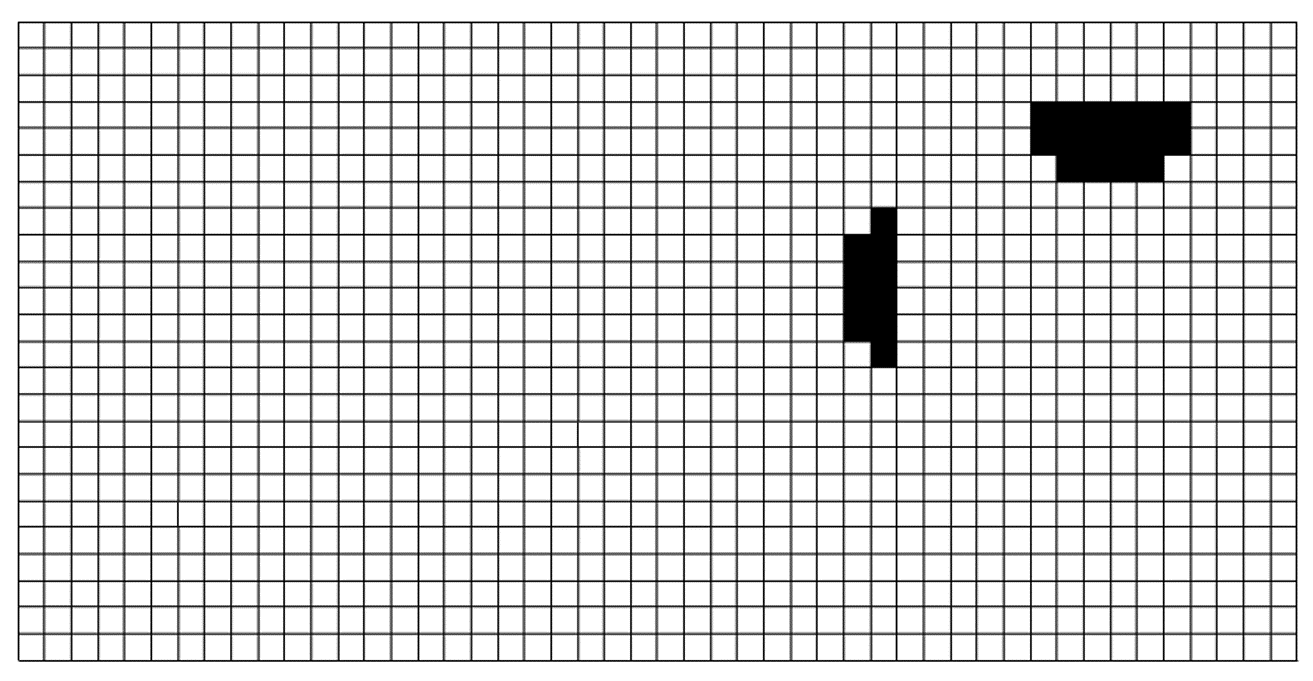
\includegraphics[width=.7\textwidth]{Pictures/Voxels/Load.png}
\vspace*{-2mm}
\caption{Load voxels}
\end{figure}
\end{minipage}
\end{frame}

\begin{frame}{Topology Optimization Process\textsuperscript{1}}
\begin{overlayarea}{\textwidth}{.8\textheight}
\begin{tikzpicture} [remember picture,overlay]
		\uncover<1->{
		\node[anchor=north,inner sep=0pt] [xshift=5cm,yshift=-0cm] (N1)
                {Provide geometry as voxel grid};
		}     
        \uncover<2->{
        \node [below =of N1, inner sep=0pt](N2){Calculate stress on each voxel};
        \draw[thick,->] (N1) -- (N2);
		}
		\uncover<3->{
		\node [right =of N2, xshift=2.5cm, inner sep=0pt](N3){};
		\node [below =of N3, yshift=-3.2cm, inner sep=0pt](N4){};
		\node [left =of N4, xshift=-2.0cm, inner sep=0pt](N5){If stress below threshold, remove voxel};
        \draw[thick,->] (N2) -- (N3) -- (N4) -- (N5);
		}
		\uncover<4->{
		\node [left =of N5, xshift=-1.3cm, inner sep=0pt](N6){};
		\node [left =of N2, xshift=-2cm, inner sep=0pt](N7){};
        \draw[thick,->] (N5) -- (N6) -- (N7) -- (N2);
		}
		\uncover<4->{
			\only<4>{
			\node [below =of N2, xshift=0.5cm, yshift=1cm](Picture){
				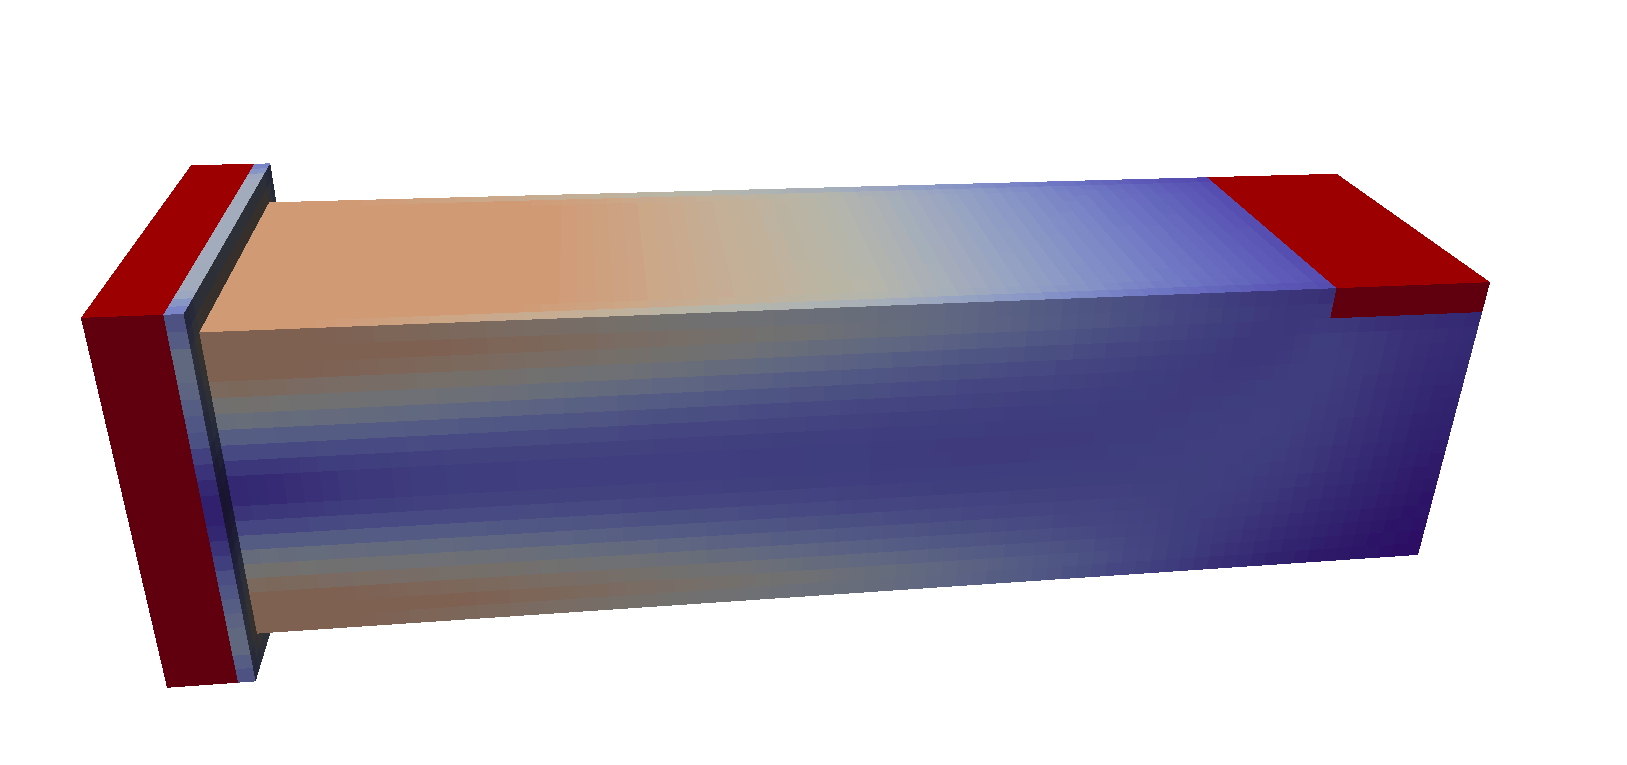
\includegraphics[scale=0.13]{Pictures/SecondHalf/Topology/Cantilever_Topy_0.png}
				};
			}	
			\only<5>{
			\node [below =of N2, xshift=0.5cm, yshift=1cm](Picture){
				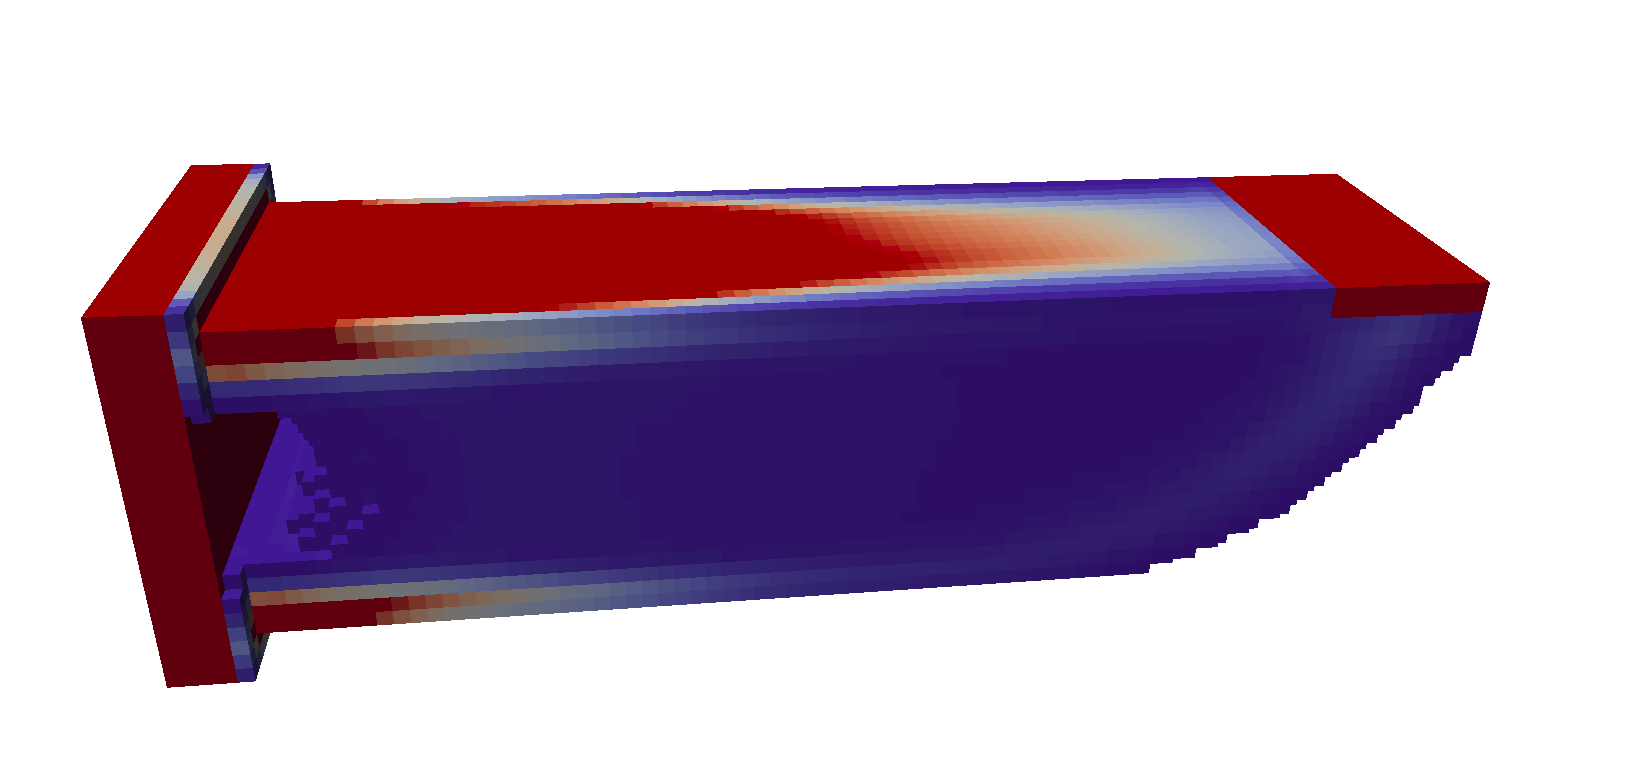
\includegraphics[scale=0.13]{Pictures/SecondHalf/Topology/Cantilever_Topy_1.png}
				};
			}	
			\only<6>{
			\node [below =of N2, xshift=0.5cm, yshift=1cm](Picture){
				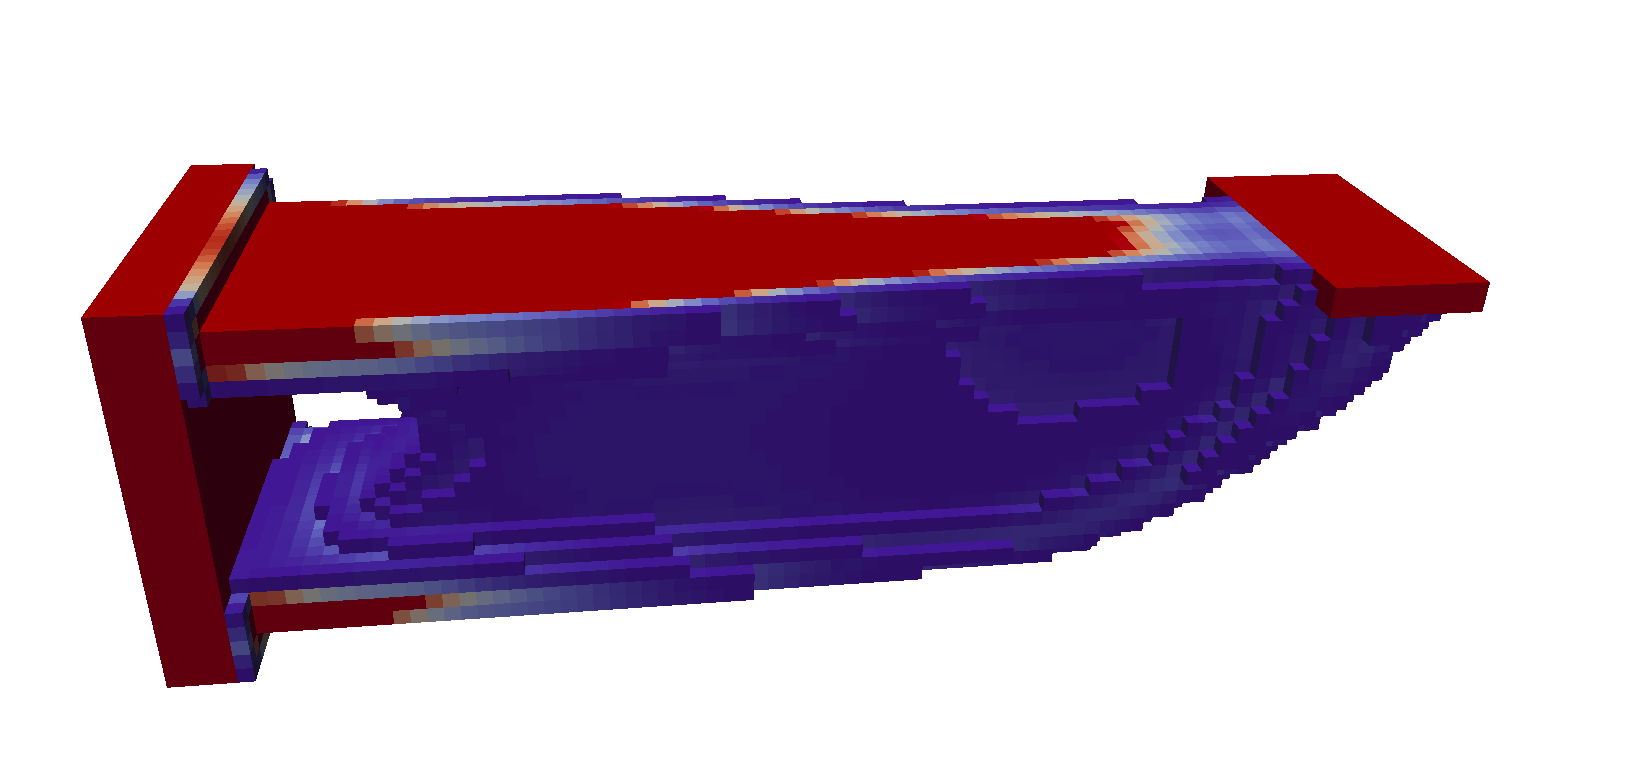
\includegraphics[scale=0.13]{Pictures/SecondHalf/Topology/Cantilever_Topy_2.png}
				};
			}	
			\only<7>{
			\node [below =of N2, xshift=0.5cm, yshift=1cm](Picture){
				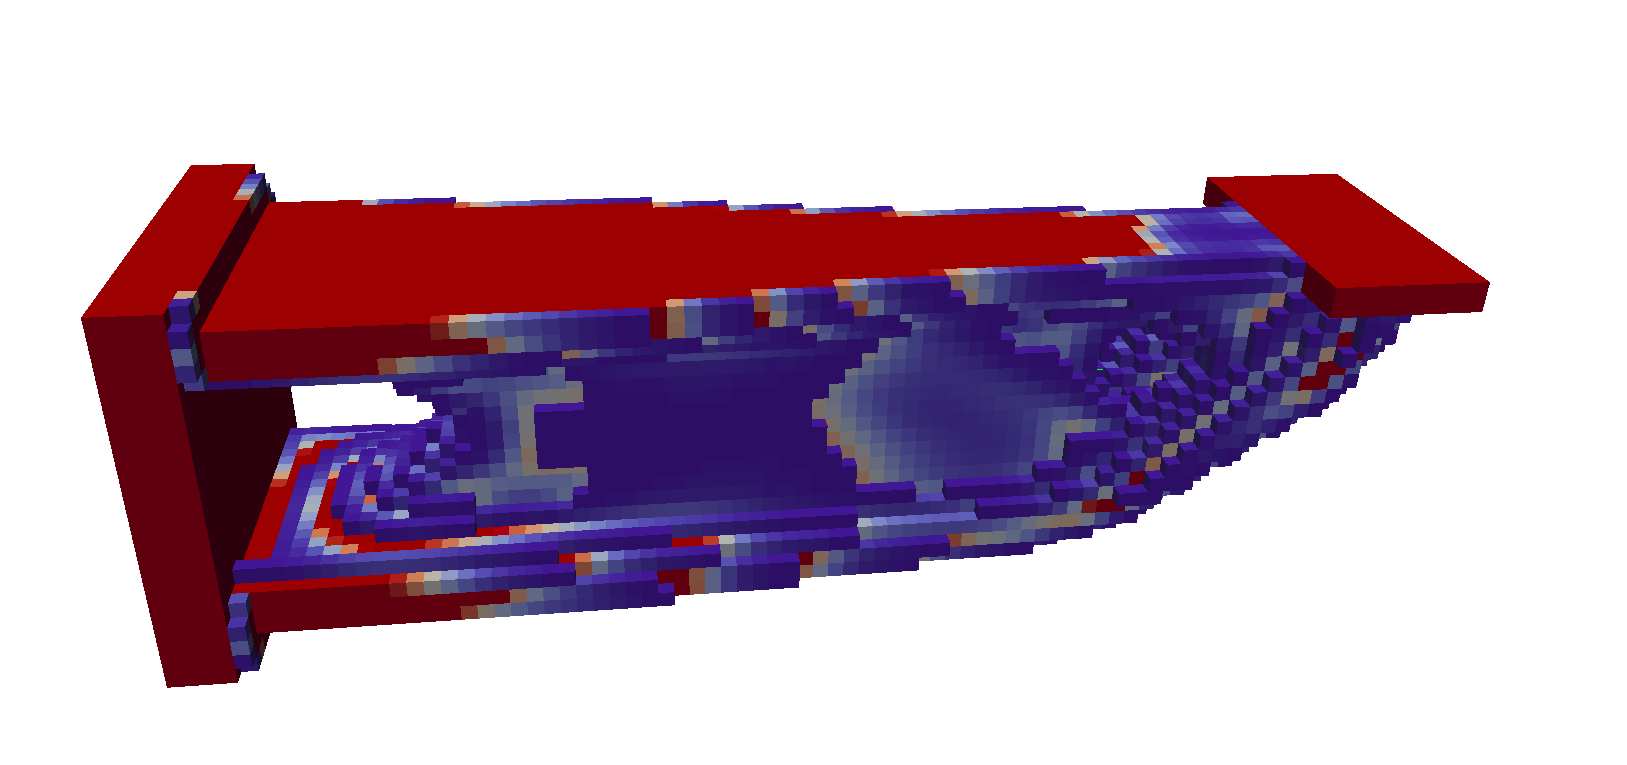
\includegraphics[scale=0.13]{Pictures/SecondHalf/Topology/Cantilever_Topy_3.png}
				};
			}	
			\only<8>{
			\node [below =of N2, xshift=0.5cm, yshift=1cm](Picture){
				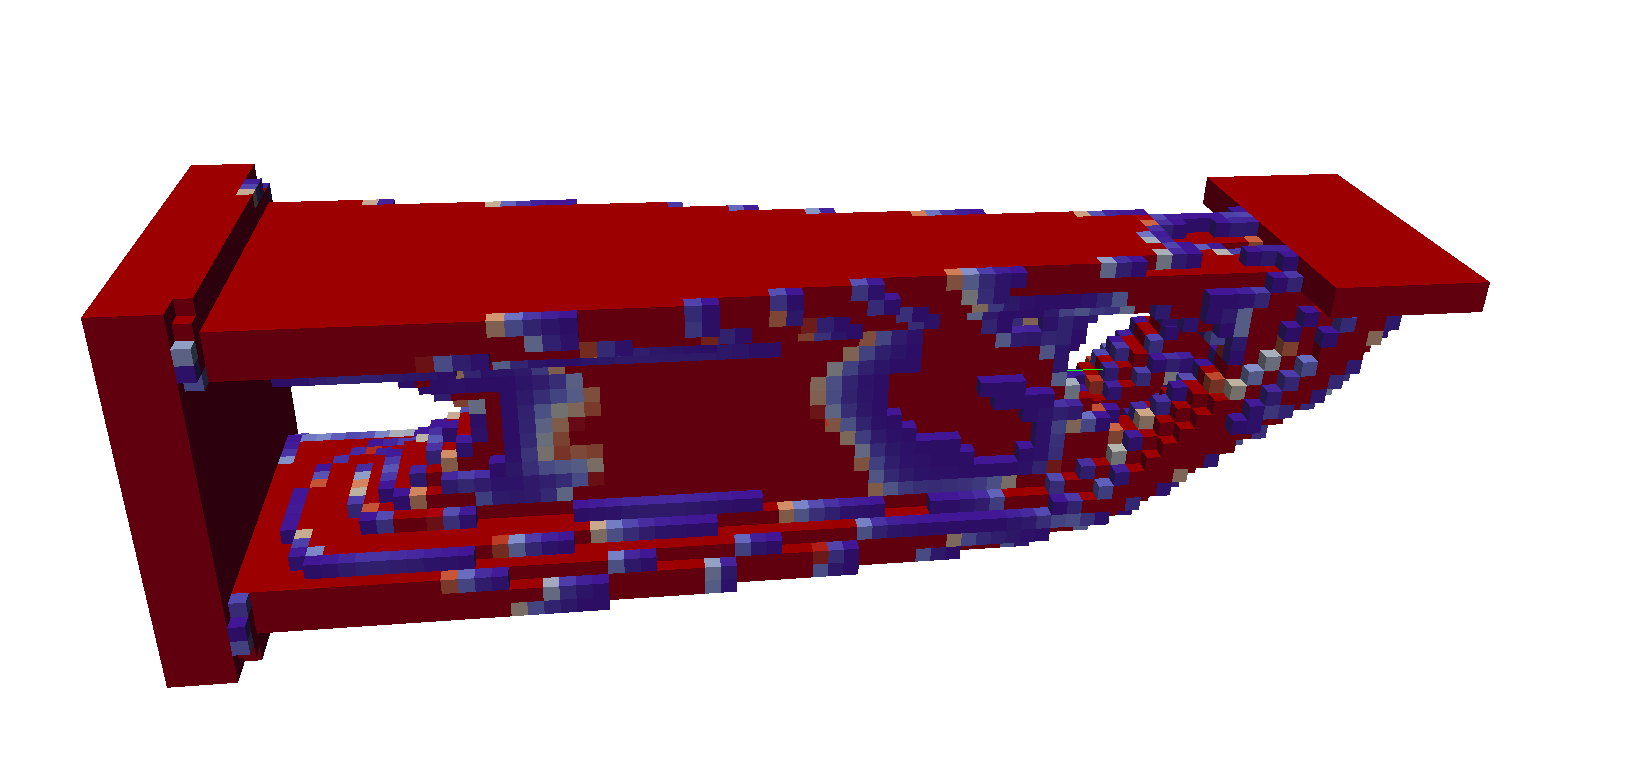
\includegraphics[scale=0.13]{Pictures/SecondHalf/Topology/Cantilever_Topy_4.png}
				};
			}	
			\only<9>{
			\node [below =of N2, xshift=0.5cm, yshift=1cm](Picture){
				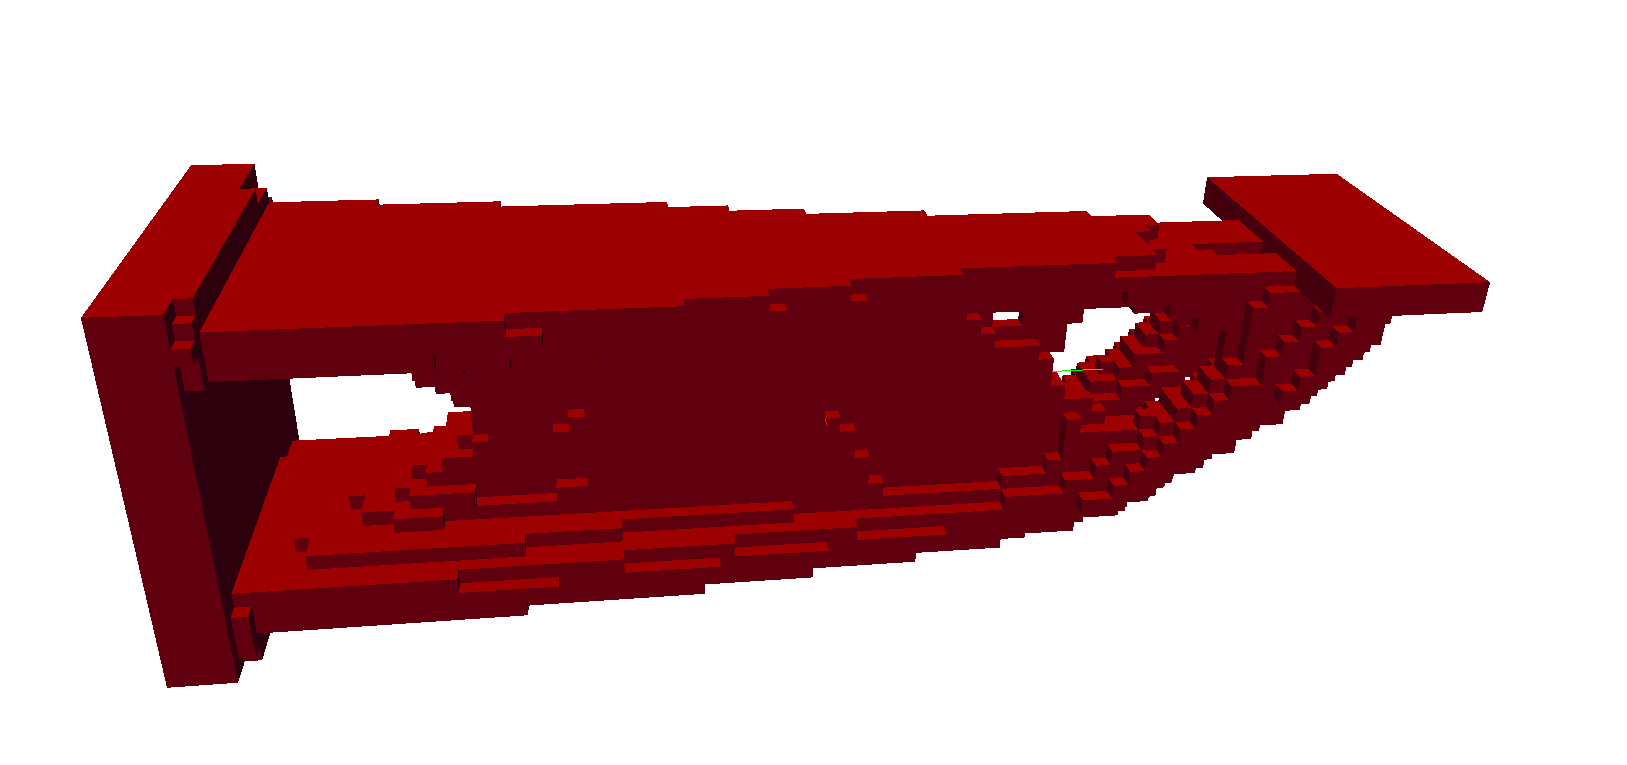
\includegraphics[scale=0.13]{Pictures/SecondHalf/Topology/Cantilever_Topy_5.png}
				};
			}	
		}
\end{tikzpicture}
\end{overlayarea}
\end{frame}

%\begin{frame}{Topology Optimization Process}
%\begin{center}
%Provide geometry as voxel grid
%$$\downarrow$$
%Calculate stress on each voxel
%$$\downarrow$$
%Remove voxel from active geometry if stress is below threshold
%\end{center}
%\end{frame}
%
%\begin{frame}{Topology Optimization Example}
%\only<1>{
%\begin{figure}
%\centering
%%\vspace{-0.5cm}
%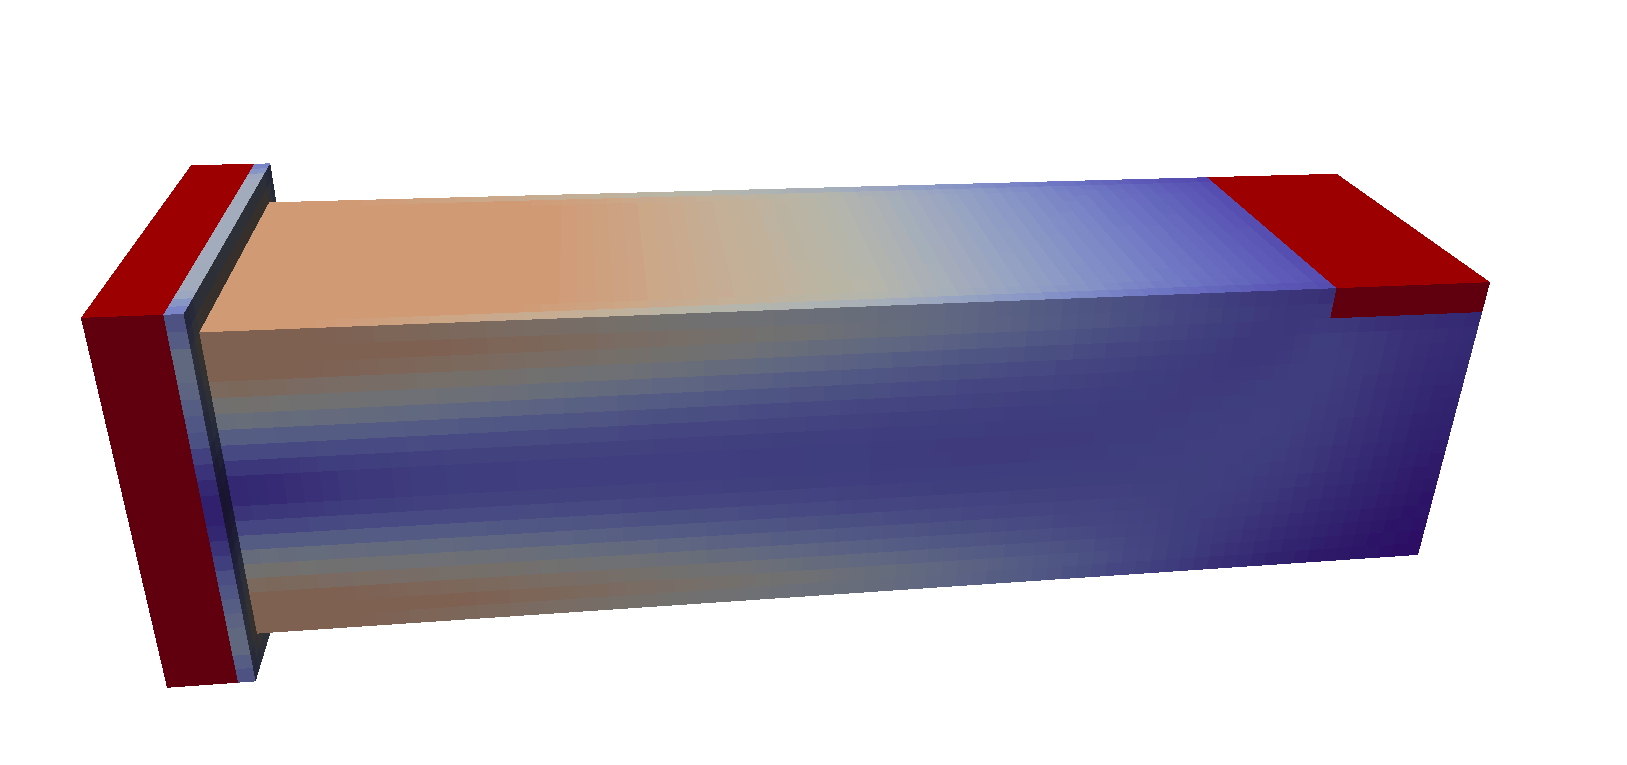
\includegraphics[width=1\textwidth]{Pictures/SecondHalf/Topology/Cantilever_Topy_0.png}
%\end{figure}}
%\only<2>{
%\begin{figure}
%\centering
%%\vspace{-0.5cm}
%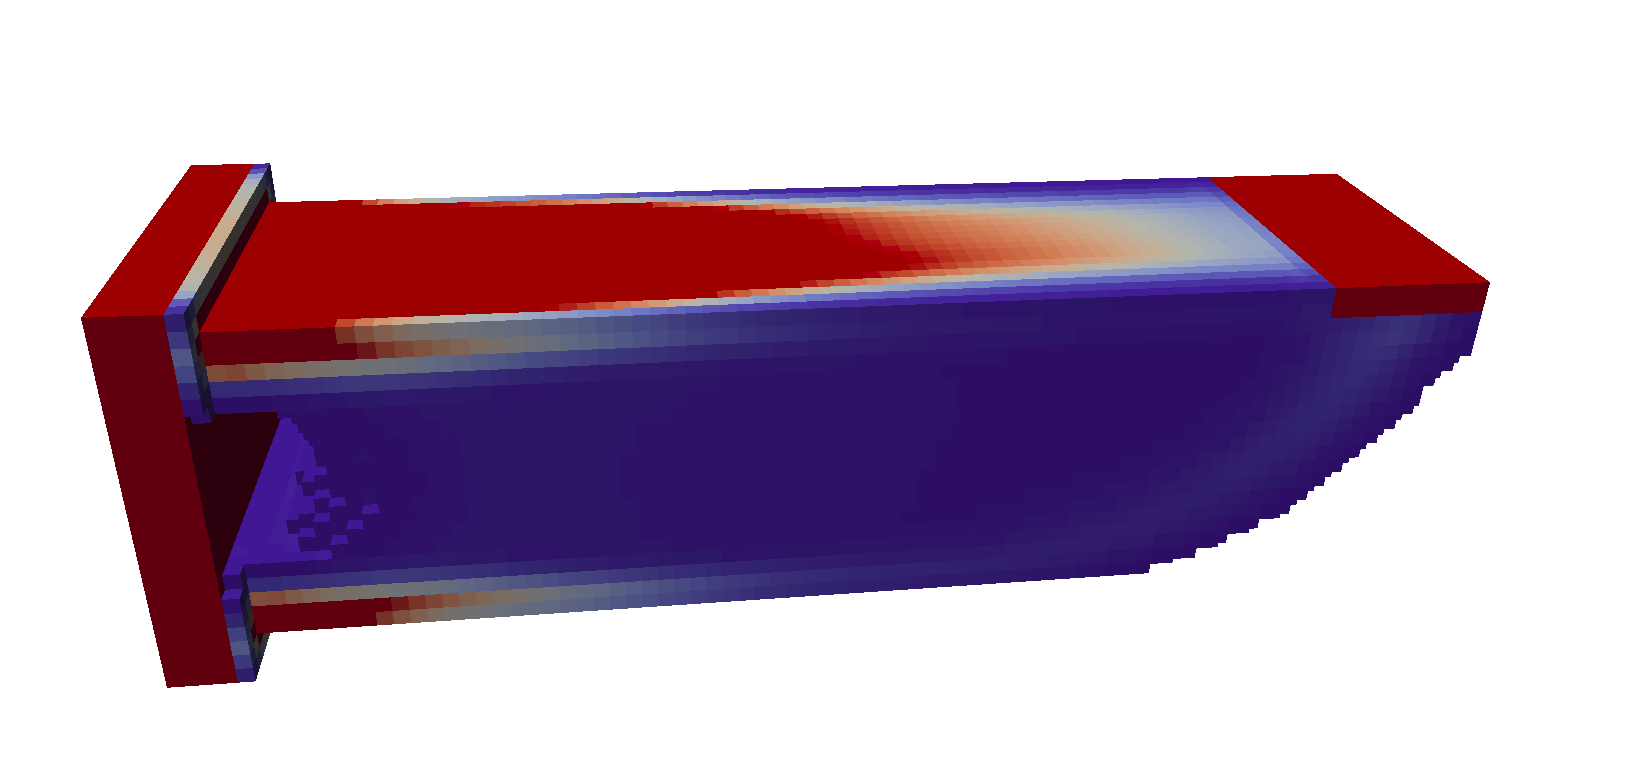
\includegraphics[width=1\textwidth]{Pictures/SecondHalf/Topology/Cantilever_Topy_1.png}
%\end{figure}}
%\only<3>{
%\begin{figure}
%\centering
%%\vspace{-0.5cm}
%\includegraphics[width=1\textwidth]
%{Pictures/SecondHalf/Topology/Cantilever_Topy_2.png}
%\end{figure}}
%\only<4>{
%\begin{figure}
%\centering
%%\vspace{-0.5cm}
%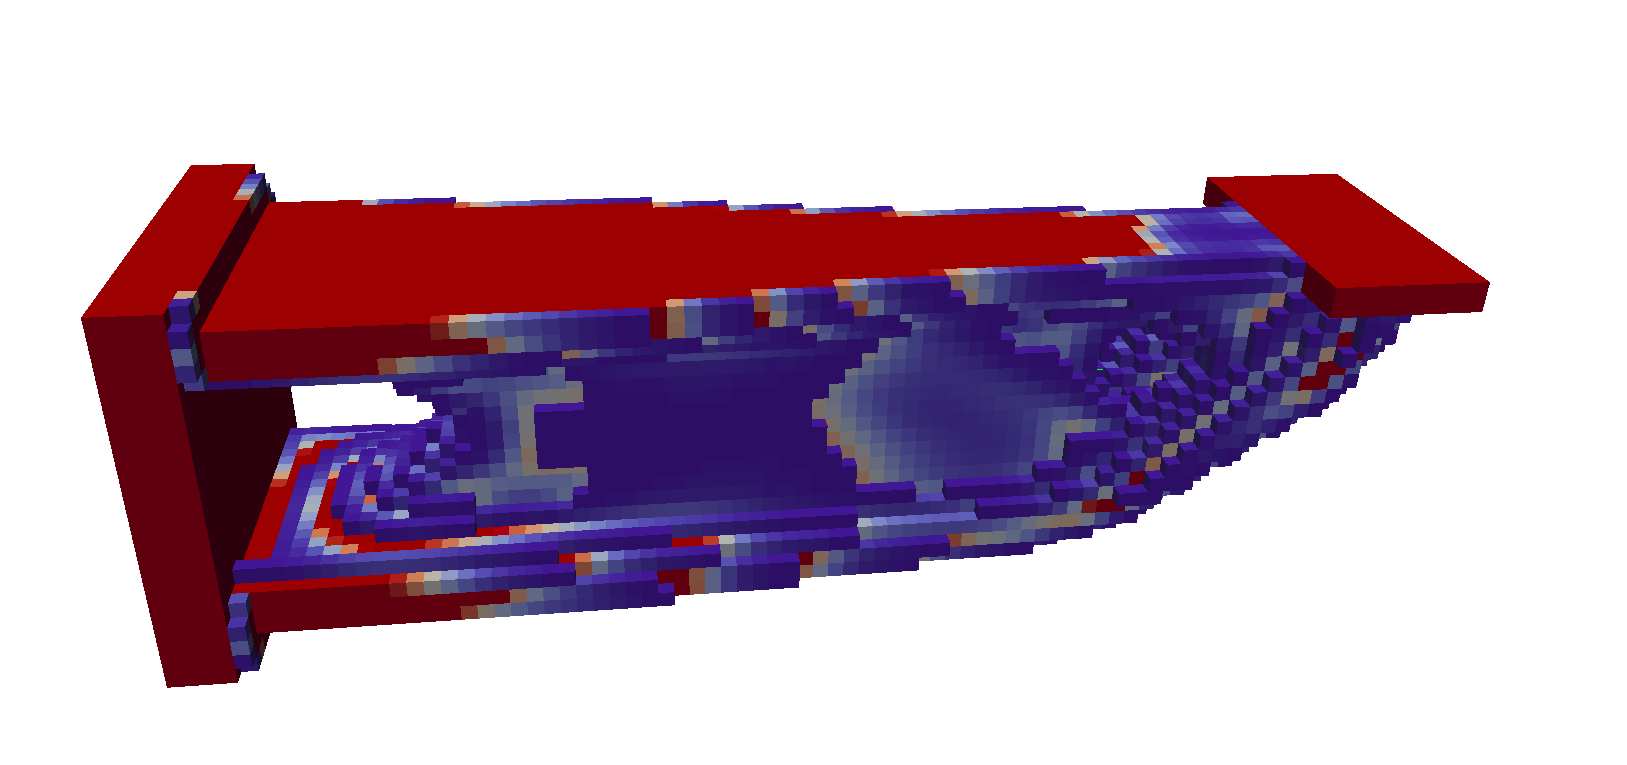
\includegraphics[width=1\textwidth]{Pictures/SecondHalf/Topology/Cantilever_Topy_3.png}
%\end{figure}}
%\only<5>{
%\begin{figure}
%\centering
%%\vspace{-0.5cm}
%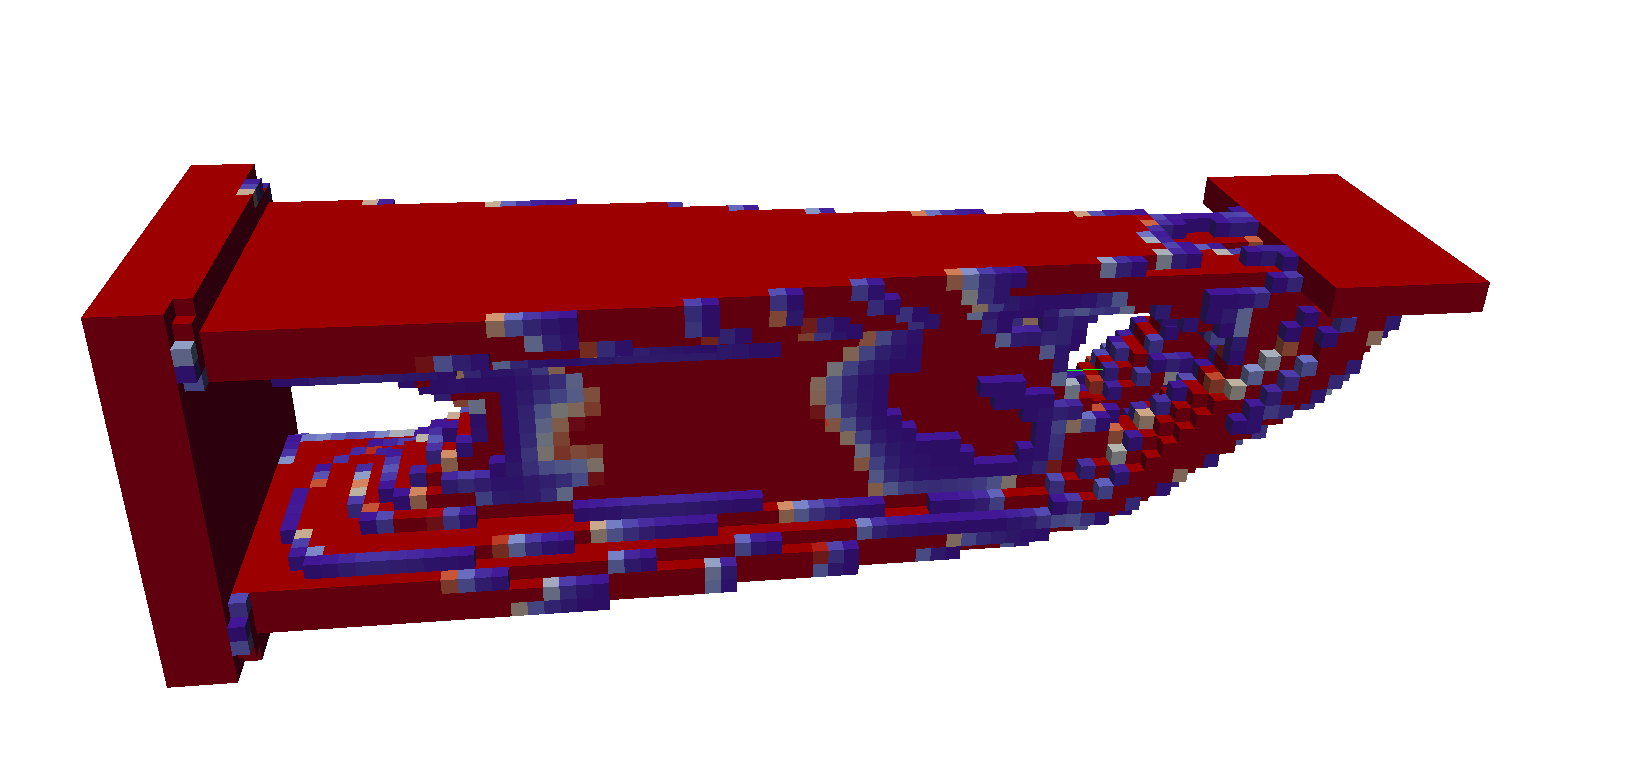
\includegraphics[width=1\textwidth]{Pictures/SecondHalf/Topology/Cantilever_Topy_4.png}
%\end{figure}}
%\only<6>{
%\begin{figure}
%\centering
%%\vspace{-0.5cm}
%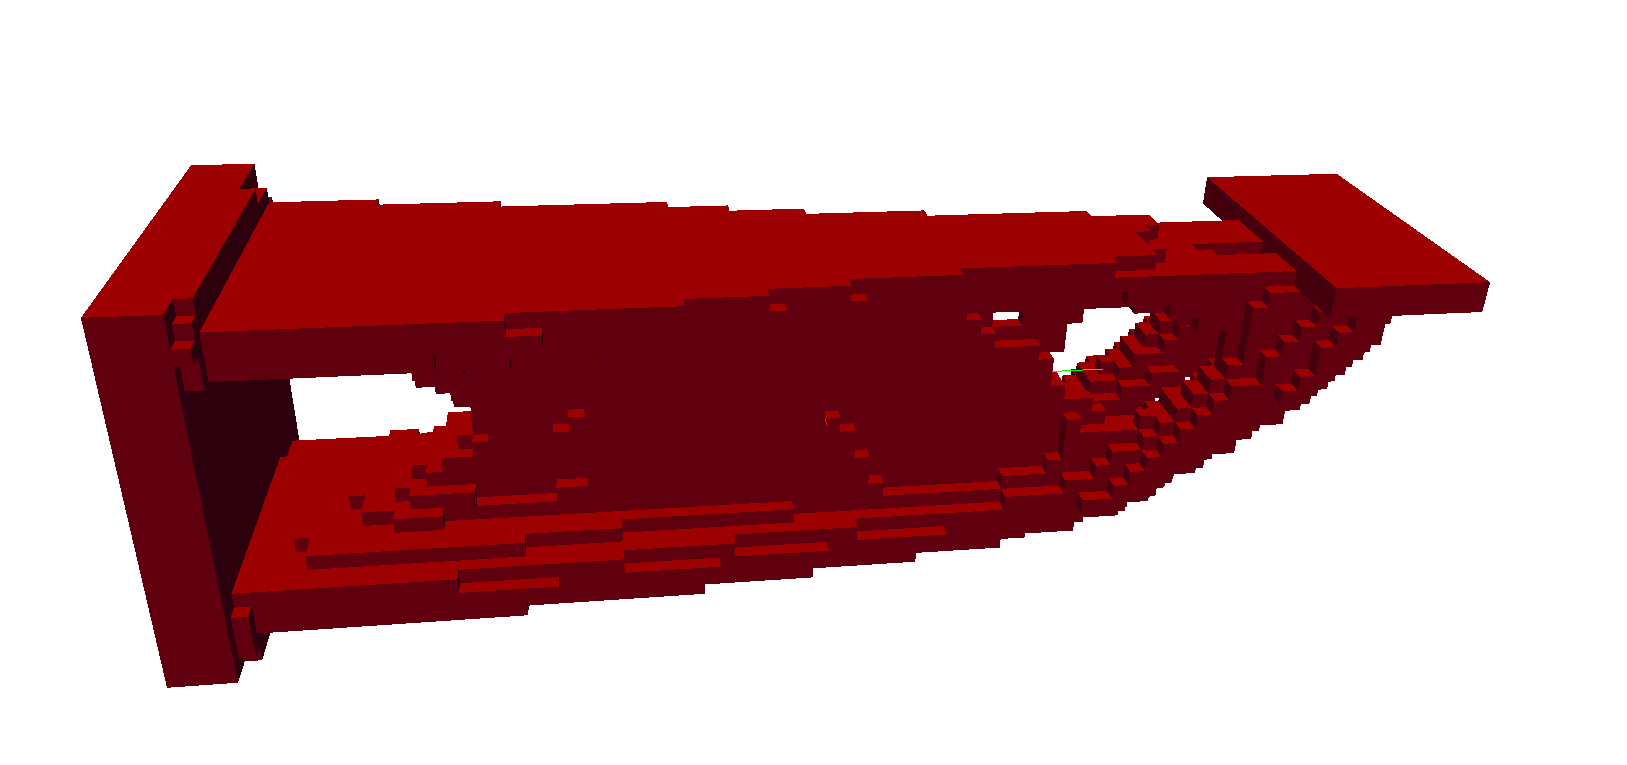
\includegraphics[width=1\textwidth]{Pictures/SecondHalf/Topology/Cantilever_Topy_5.png}
%\end{figure}}
%\end{frame}


\section{Feature recognition}

\begin{frame}

	\frametitle{From Voxel to Mesh Geometry}
	\begin{minipage}{0.85\textwidth}
		\begin{itemize}
		\item Extract isosurface from voxel information
		\end{itemize}

		\begin{itemize}
		\item Algorithms: Marching Cubes, Dual Contouring, Extended Models
		\end{itemize}

		\begin{figure}
		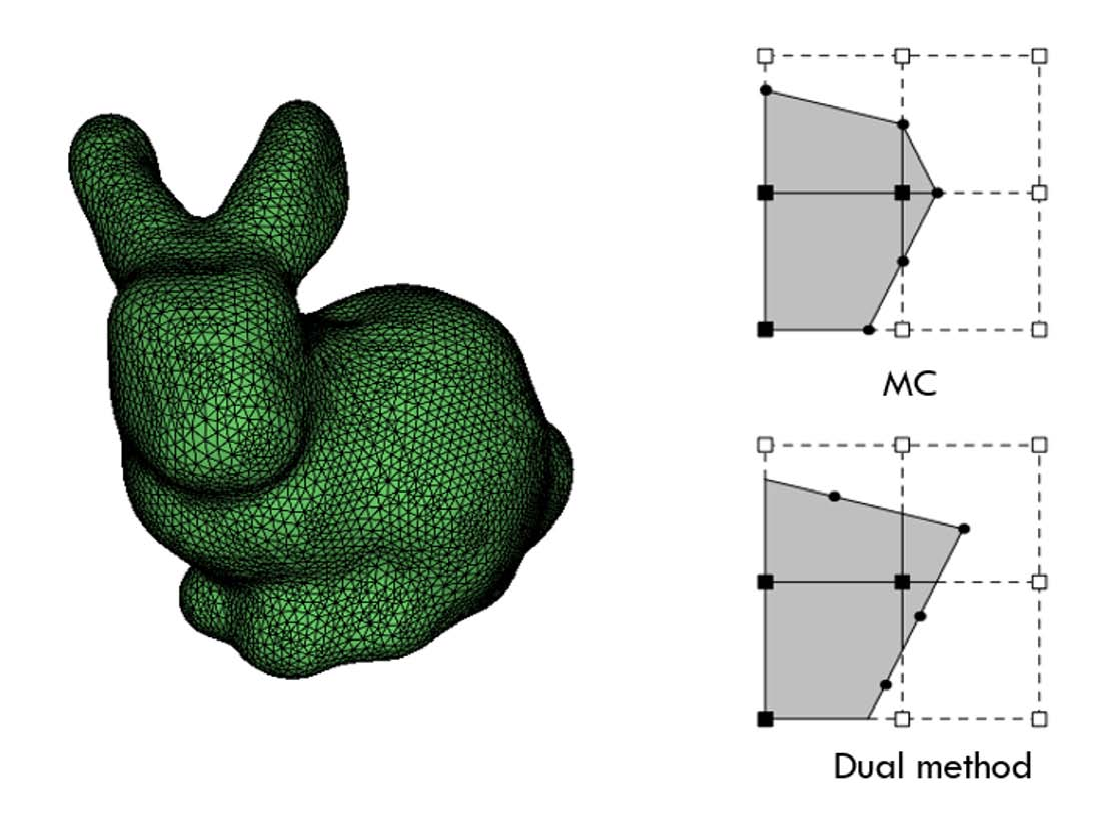
\includegraphics[scale=0.4]{Pictures/bunny_MC.pdf}

		\end{figure}

	\end{minipage}
	\begin{minipage}{0.14\textwidth}
		\begin{figure}
					\scalebox{0.08}{
\includegraphics{Pictures/1CAD.pdf}}\\
					\scalebox{0.08}{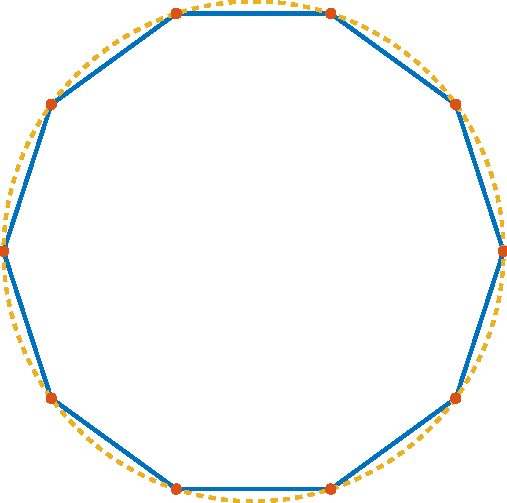
\includegraphics{Pictures/2STL.pdf}}\\
					\scalebox{0.08}{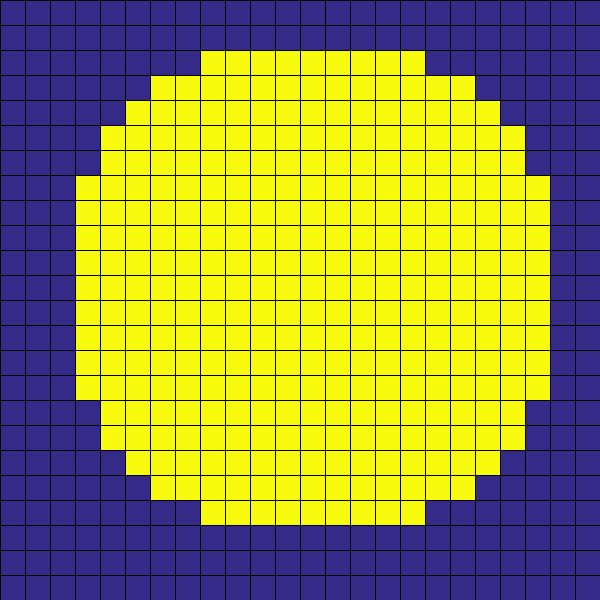
\includegraphics{Pictures/3VOX.pdf}}\\
					\scalebox{0.08}{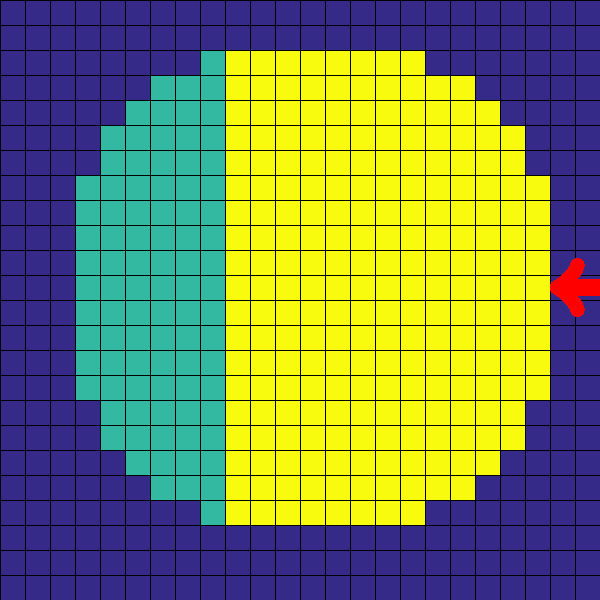
\includegraphics{Pictures/4TPD.pdf}}\\
					\scalebox{0.08}{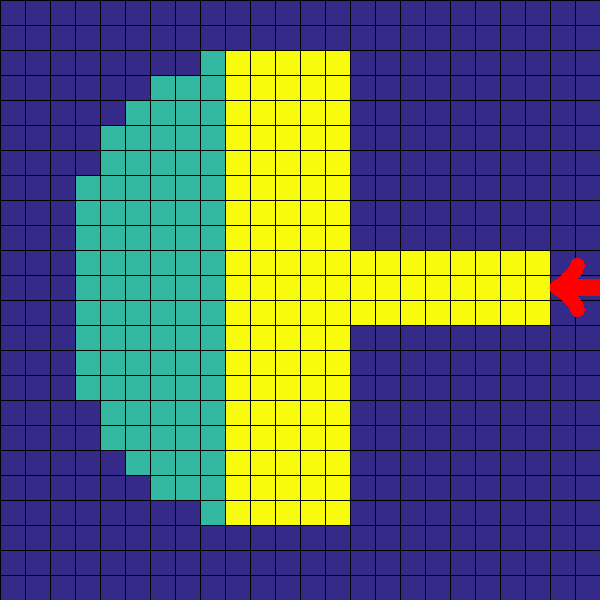
\includegraphics{Pictures/5TOPOPT.pdf}}\\
					\scalebox{0.08}{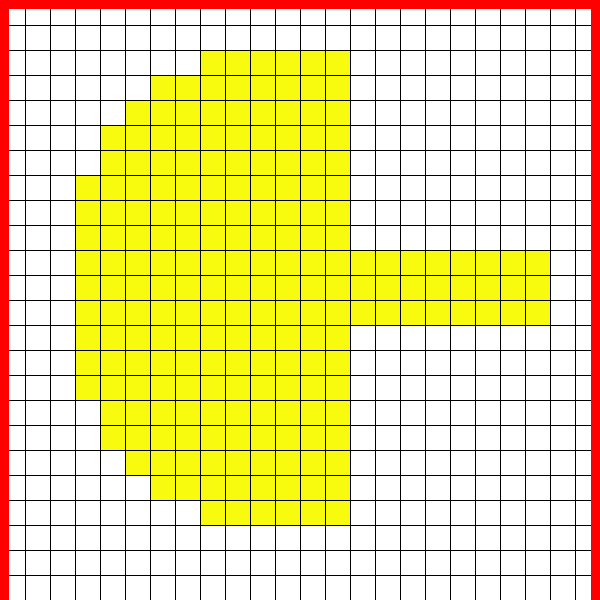
\includegraphics{Pictures/6TOPYOUTmark2.pdf}}\\
					\scalebox{0.08}{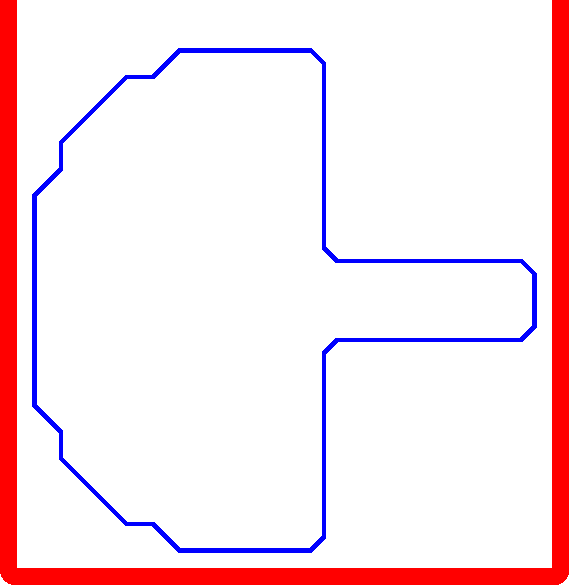
\includegraphics{Pictures/7MCmark1.pdf}}  %THIS NEEDS TO BE CHANGED FOR MARK!
		\end{figure}
	\end{minipage}



\end{frame}

\begin{frame}

	\frametitle{Surface Extraction}
	\begin{minipage}{0.85\textwidth}
	\text Contour Filtering using Implicit Modelling 


	\begin{figure}
	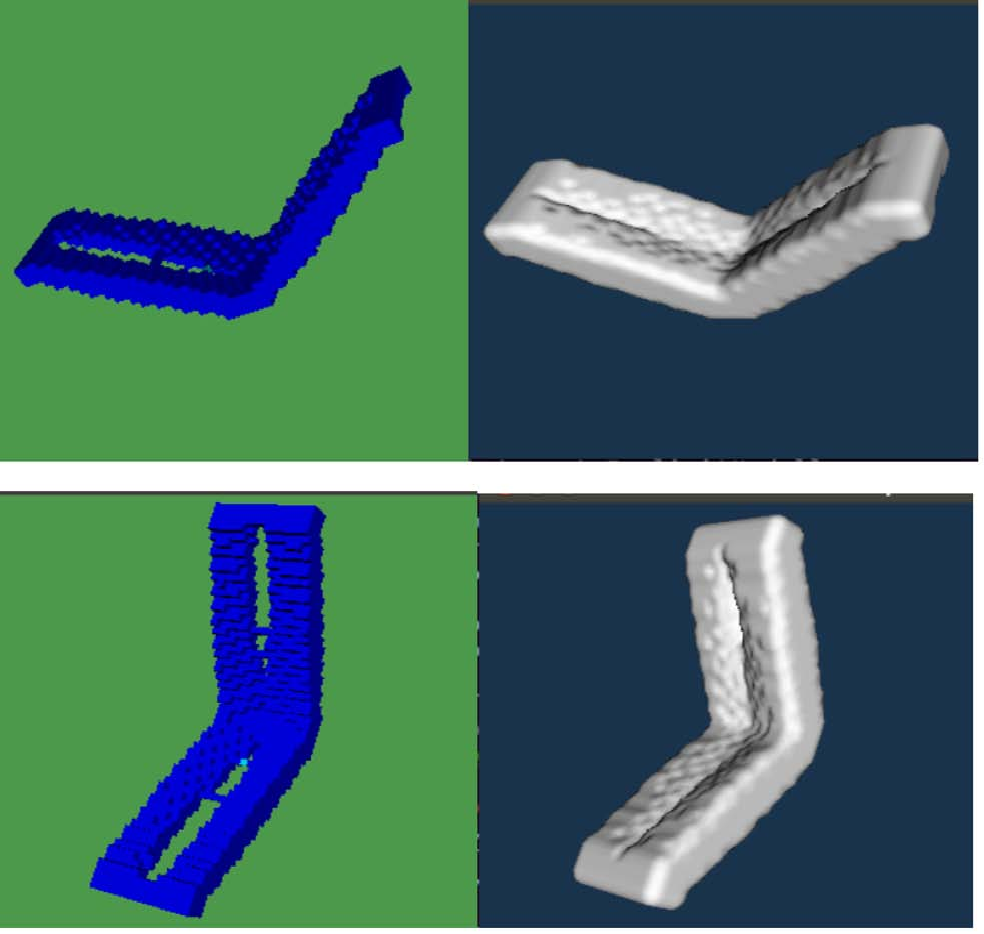
\includegraphics[scale=0.35]{Pictures/contouring.pdf}

	\end{figure}


	\textbf {Problem: Holes are not taken into account}

	\end{minipage}
	\begin{minipage}{0.14\textwidth}
		\begin{figure}
					\scalebox{0.08}{
\includegraphics{Pictures/1CAD.pdf}}\\
					\scalebox{0.08}{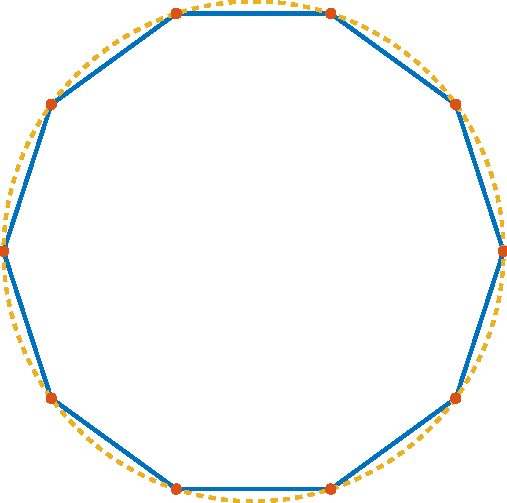
\includegraphics{Pictures/2STL.pdf}}\\
					\scalebox{0.08}{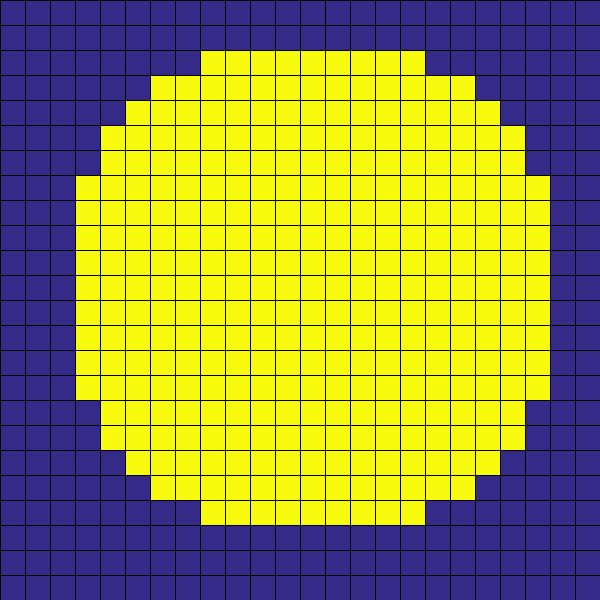
\includegraphics{Pictures/3VOX.pdf}}\\
					\scalebox{0.08}{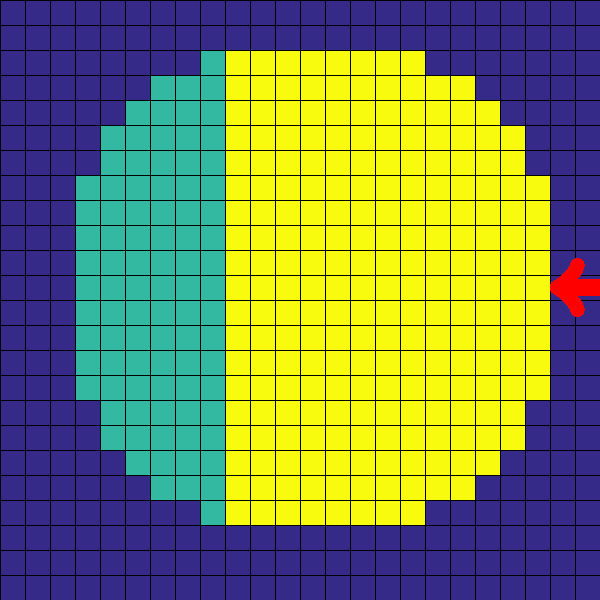
\includegraphics{Pictures/4TPD.pdf}}\\
					\scalebox{0.08}{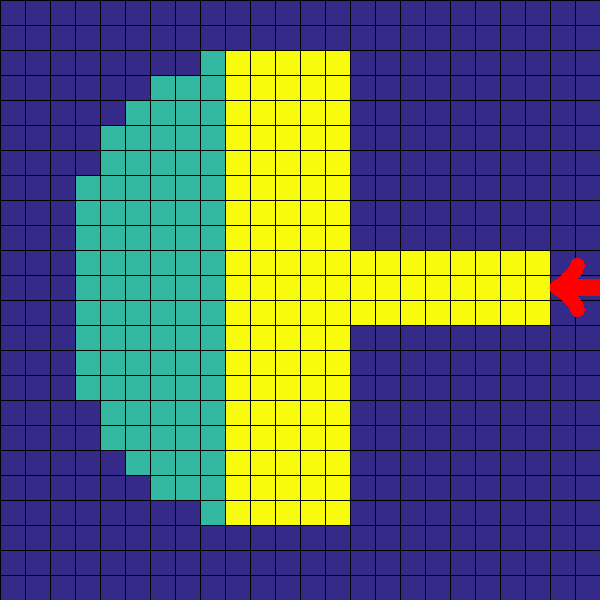
\includegraphics{Pictures/5TOPOPT.pdf}}\\
					\scalebox{0.08}{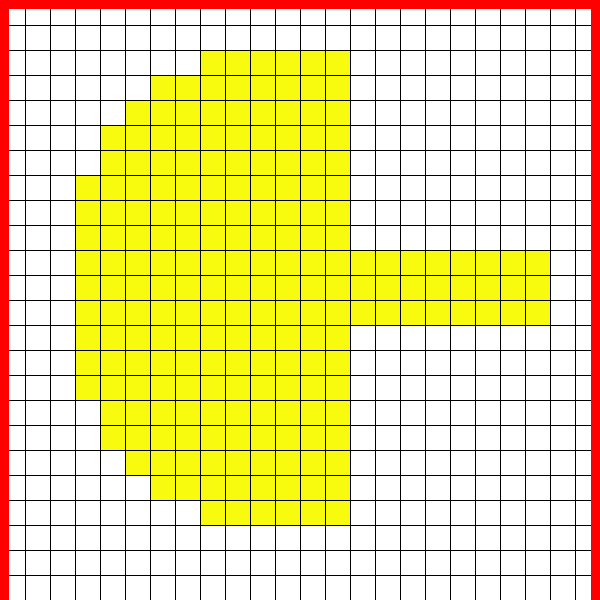
\includegraphics{Pictures/6TOPYOUTmark2.pdf}}\\
					\scalebox{0.08}{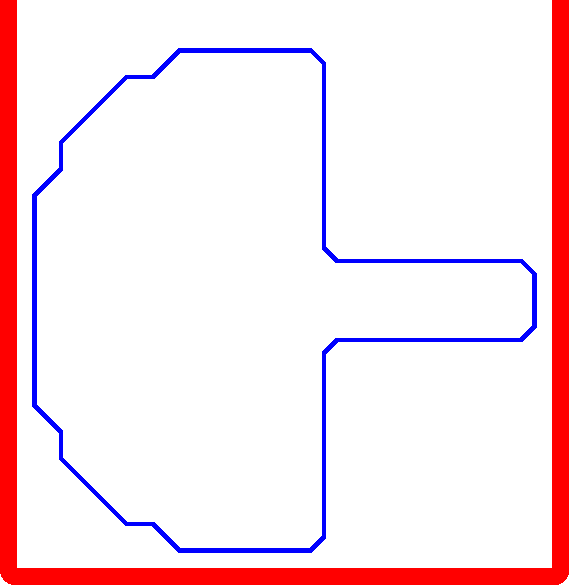
\includegraphics{Pictures/7MCmark1.pdf}}  %THIS NEEDS TO BE CHANGED FOR MARK!
		\end{figure}
	\end{minipage}





\end{frame}

\begin{frame}

	\frametitle{Decimation}
	\begin{minipage}{0.85\textwidth}
	\begin{itemize}
	\item Fine mesh to a coarser mesh through Decimation- Reduction of number of triangles. (Upper: 50\% Lower: 90\% )
	\end{itemize}

	\begin{itemize}
	\item Smoothing step is needed in between
	\end{itemize}

	\begin{figure}
	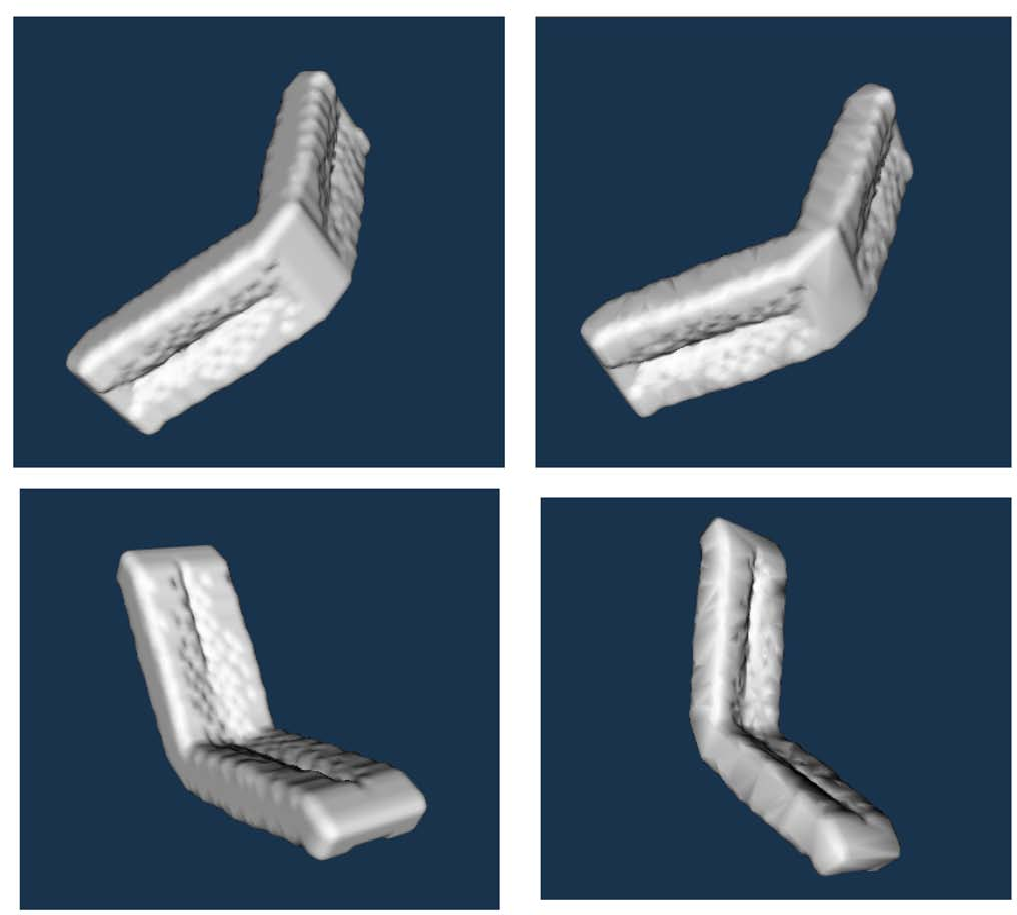
\includegraphics[scale=0.34]{Pictures/Decimation.pdf}

	\end{figure}
	\end{minipage}
	\begin{minipage}{0.14\textwidth}
		\begin{figure}
					\scalebox{0.08}{
\includegraphics{Pictures/1CAD.pdf}}\\
					\scalebox{0.08}{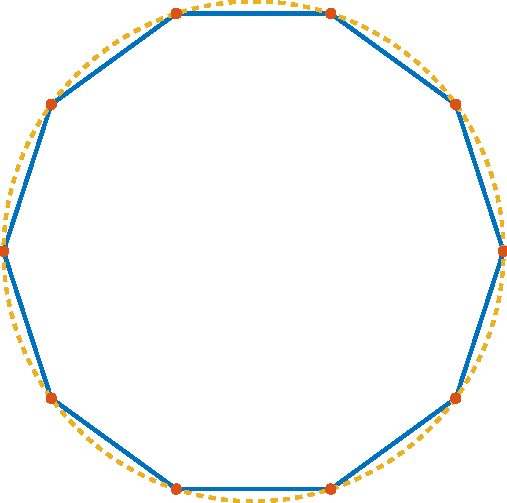
\includegraphics{Pictures/2STL.pdf}}\\
					\scalebox{0.08}{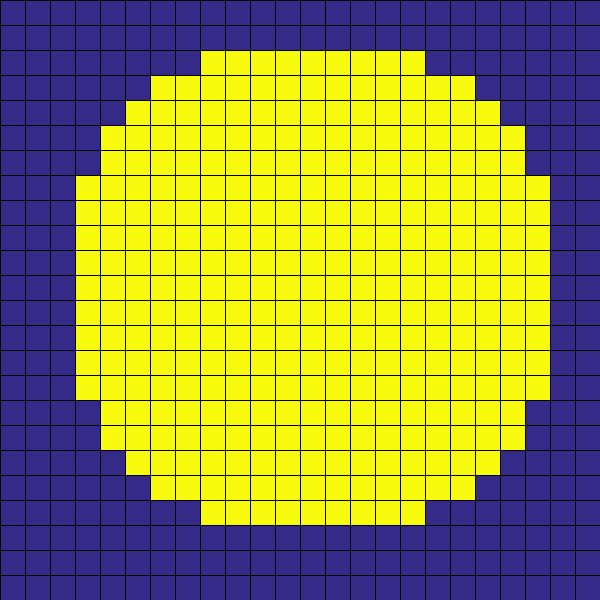
\includegraphics{Pictures/3VOX.pdf}}\\
					\scalebox{0.08}{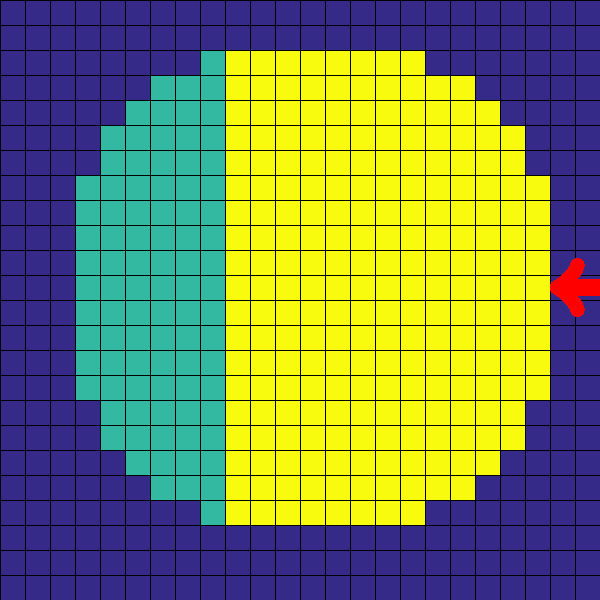
\includegraphics{Pictures/4TPD.pdf}}\\
					\scalebox{0.08}{\includegraphics{Pictures/5TOPOPT.pdf}}\\
					\scalebox{0.08}{\includegraphics{Pictures/6TOPYOUTmark2.pdf}}\\
					\scalebox{0.08}{\includegraphics{Pictures/7MCmark1.pdf}}  %THIS NEEDS TO BE CHANGED FOR MARK!
		\end{figure}
	\end{minipage}





\end{frame}


\end{document}
